\documentclass[conference]{./IEEEtran/IEEEtran}
\usepackage{color}
\usepackage{listings}
\definecolor{mygreen}{rgb}{0,0.6,0}
\definecolor{mygray}{rgb}{0.5,0.5,0.5}
\definecolor{mymauve}{rgb}{0.58,0,0.82}
\usepackage{makecell}
\usepackage{enumitem}
\renewcommand\theadfont{\bfseries}
\newcommand{\tableWifiDevices}{
\begin{table}[H]
	\centering
	\caption{Wi-Fi Devices.}\label{tbl:WifiDevices}
	\makebox[\textwidth][c]{\begin{tabular} {| c | c | c | c | c | c |}
		\hline
		\thead{ID} & \thead{Manuf} & \thead{Device Type} & \thead{Device Name} &  \thead{MAC} & \thead{IP Address} \\ 
		\hline
		w$_1 $ & Calix & Wireless Router & Moria & EC:4F:82:73:D1:1A & - \\
		\hline
		w$_2 $ & Belkin & Camera & NetCam & EC:1A:59:E4:FD:41 & 192.168.1.44 \\
		\hline
		w$_3 $ & Belkin & Outlet & Switch1 & B4:75:0E:0D:33:D5 & 192.168.1.40 \\
		\hline
		w$_4 $ & Belkin & Outlet & Switch2 & B4:75:0E:0D:94:65 & 192.168.1.41 \\
		\hline
		w$_5 $ & Belkin & Outlet & Switch3 & 94:10:3E:2B:7A:55 & 192.168.1.42 \\
		\hline
		w$_6 $ & Belkin & Outlet & Switch4 & 14:91:82:C8:6A:09 & 192.168.1.7 \\
		\hline
		w$_7 $ & Belkin & Motion Sensor & Motion & EC:1A:59:F1:FB:21 & 192.168.1.43 \\
		\hline
		w$_8 $ & Belkin & Outlet & Insight & 14:91:82:24:DD:35 & 192.168.1.47 \\
		\hline
		w$_9 $ & WeMo & Outlet & Mini & 60:38:E0:EE:7C:E5 & 192.168.1.51 \\
		\hline
		w$_{10} $ & Raspberry Pi 3B & Computer & Pi & B8:27:EB:09:1A:81 & 12.168.1.50 \\
		\hline
		w$_{11} $ & Apple & iPhone 6+ & Steves-phone & A0:18:28:33:34:F8 & 192.168.1.4 \\
		\hline
		w$_{12} $ & Apple & TV 2 & Apple-TV & 08:66:98:ED:1E:19 & 192.168.1.54 \\
		\hline
	\end{tabular}}
\end{table}
}

\newcommand{\tableWifiDeviceShort}{
	\begin{table}[tbp]
		\centering
		\caption{Wi-Fi Devices.}\label{tbl:WifiDevicesShort}
			\begin{tabular} {| c | c | c | c |}
				\hline
				\thead{ID} & \thead{Manuf} & \thead{Device Type} & \thead{Device Name} \\ 
				\hline
				w$_1 $ & Calix & Wireless Router & Prancing Pony  \\
				\hline
				w$_{2-5} $ & Belkin & Outlet & Switch1-4 \\
				\hline
				w$_6 $ & WeMo & Outlet & Mini  \\
				\hline
				w$_7 $ & Belkin & Outlet & Insight  \\
				\hline
				w$_8 $ & Belkin & Motion Sensor & Motion \\
				\hline
				w$_9 $ & Belkin & Camera & NetCam  \\
				\hline
				w$_{10} $ & Raspberry Pi 3B & Computer & Pi \\
				\hline
				w$_{11} $ & Apple & iPhone 6+ & Steves-phone  \\
				\hline
				w$_{12} $ & Apple & TV 2 & Apple-TV \\
				\hline
			\end{tabular}
	\end{table}
}

\newcommand{\tableBtleDevicesShort}{
	\begin{table}[tbp]
		\centering
		\caption{BLE Devices.}\label{tbl:BtleDevicesShort}
\begin{tabular}{|c|c|c|c|}
	\hline
	\thead{ID} & \thead{Manuf} & \thead{Device Type} & \thead{Device Name} \\
	\hline
	b$ _1 $ & Elgato & Indoor Temperature & Eve Room \\
	\hline
	b$ _2 $ & Elgato & Outdoor Temperature & Eve Weather \\
	\hline
	b$ _3 $ & Elgato & Motion Sensor & Eve Motion \\
	\hline
	b$ _4 $ & Elgato & Outlet & Eve Energy \\
	\hline
	b$ _5 $ & Elgato & Door Sensor & Eve Door \\
	\hline
	b$ _6 $ & Instant Pot & Smart Cooker & Instant Pot \\
	\hline
	b$ _7 $ & MPow & Lightbulb & Playbulb \\
	\hline
	b$ _8 $ & ZKTeco & Lock & BioLock \\
	\hline
	b$ _{9} $ & BitLock & Lock & Bike lock \\
	\hline
	b$ _{10} $ & SafeTech & Gunsafe & Gunsafe \\
	\hline
	b$ _{11} $ & Apple & iPhone 6+ & Steves-phone \\
	\hline
	b$ _{12} $ & Apple & TV 2 & Apple TV \\
	\hline
\end{tabular}
\end{table}
}

\newcommand{\tableDeviceClassifier}{
	\begin{table*}[tbp]
		\centering
		\caption{Classifier Criterion.}\label{tbl:DeviceClassifier}
		\begin{tabular} {| c | c | c |}
			\hline
			\thead{Device Type} & \thead{Device Classification} & \begin{tabular}{@{}c@{}}\thead{Event Identification} \\ (Relies on Device Classification)\end{tabular} \\
			\hline
			Outlet & $FSize_{in} > 650\ bytes$ & $1,000 > FSize_{in} > 600\ bytes$ \\
			\hline
			Sensor & $device\ != outlet\ and\ all\ FSize_{in} < 275\ bytes$ & $100,000>\sum\limits_{t}^{t+1}FSize_{out}>10,000\ bytes$\\
			\hline
			Camera & $device\ != outlet\ and\ 275 < FSize_{in} < 300\ bytes$ & $\sum\limits_{t}^{t+1}FSize_{out}>100,000\ bytes$\\
			\hline
		\end{tabular}
	\end{table*}
}

\newcommand{\tableBtleDevices}{
\begin{table}[H]
	\centering
	\caption{BLE Devices.}\label{tbl:BtleDevices}
	\makebox[\textwidth][c]{\begin{tabular}{| c | c|c|c|}
		\hline
		\thead{ID} & \thead{Manuf} & \thead{Device Type} & \thead{Device Name} \\
		\hline
		b$ _1 $ & Elgato & Indoor Temperature & Eve Room \\
		\hline
		b$ _2 $ & Elgato & Outdoor Temperature & Eve Weather \\
		\hline
		b$ _3 $ & Elgato & Motion Sensor & Eve Motion \\
		\hline
		b$ _4 $ & Elgato & Outlet & Eve Energy \\
		\hline
		b$ _5 $ & Elgato & Switch & Eve Light \\
		\hline
		b$ _6 $ & Elgato & Door Sensor & Eve Door \\
		\hline
		b$ _7 $ & Instant Pot & Smartcooker & Instant Pot \\
		\hline
		b$ _8 $ & MPow & Lightbulb & Playbulb \\
		\hline
		b$ _9 $ & ZKTeco & Lock & BioLock \\
		\hline
		b$ _{10} $ & BitLock & Lock & Bike lock \\
		\hline
		b$ _{11} $ & SafeTech & Gunsafe & Gunsafe \\
		\hline
		b$ _{12} $ & Apple & iPhone 6+ & Steves-phone \\
		\hline
		b$ _{13} $ & Apple & TV 2 & Apple TV \\
		\hline
	\end{tabular}}
\end{table}
}

\newcommand{\tablePerformanceMetrics}{
	\begin{table}[H]
		\centering
		\caption{Performance Metrics}
		\makebox[\textwidth][c]{\begin{tabular}{|c|c|c|c|}
			\hline
			\thead{Metric} & \thead{Units} & \thead{Accepted Range} & \thead{Expected Value} \\
			\hline
			DCSR (Device Classification Success Rate) & \% & 0 to 100 & $>$ 75\% \\
			\hline
			EISR (Event Identification Success Rate) & \% & 0 to 100 & $>$ 75\% \\
			\hline
			EIFP (Event Identification False Positives) & \% & 0 to 100 & $>$ 75\% \\
			\hline
			EIFN (Event Identification False Negatives) & \% & 0 to 100 & $>$ 75\% \\
			\hline
			ULSR (User Location Success Rate) & \% & 0 to 100 & $>$ 75\% \\
			\hline
			CT (Completion Time) & minutes & 0 to $\infty$ & $<$ 120 minutes \\
			\hline
			HDU (Hard Drive Usage) & bytes & 0 to $\infty$ & $<$ 20 GB \\
			\hline
		\end{tabular}}
		\label{tbl:PerformanceMetrics}
	\end{table}
}

\newcommand{\tableEvents}{
	\begin{table}[h!]
		\centering
		\caption{Experiment Events}\label{tbl:Events}
		\begin{tabular}{|c|c|c|c|}
			\hline
			\ & \thead{Device Name} & \thead{Action} & \thead{Protocol} \\
			\hline
			1 & Bike Lock & Unlock & BLE \\
			\hline
			2 & BioLock & Unlock & BLE \\
			\hline
			3 & Instant Pot & Turn on & BLE \\
			\hline
			4 & Instant Pot & Turn off & BLE \\
			\hline
			5 & Gunsafe  & Open & BLE \\
			\hline
			6 & Gunsafe  & Close & BLE \\
			\hline
			7 & Eve Room & Get temperature in living room & BLE \\
			\hline
			8 & Eve Weather & Get temperature on patio & BLE \\
			\hline
			9 & Eve Door & Open & BLE \\
			\hline
			10 & Eve Door & Close & BLE \\
			\hline
			11 & Eve Energy & Turn on & BLE \\
			\hline
			12 & Eve Energy & Turn off & BLE \\
			\hline
			13 & Eve Motion & Activate motion sensor & BLE \\
			\hline
			14 & Playbulb & Turn on & BLE \\
			\hline
			15 & Playbulb & Turn off & BLE \\
			\hline
			16 & Switch1 & Turn on & Wi-Fi \\
			\hline
			17 & Switch1 & Turn off & Wi-Fi \\
			\hline
			18 & Switch2 & Turn on & Wi-Fi \\
			\hline
			19 & Switch2 & Turn off & Wi-Fi \\
			\hline
			20 & Switch3 & Turn on & Wi-Fi \\
			\hline
			21 & Switch3 & Turn off & Wi-Fi \\
			\hline
			22 & Switch4 & Turn on & Wi-Fi \\
			\hline
			23 & Switch4 & Turn off & Wi-Fi \\
			\hline
			24 & Mini & Turn on & Wi-Fi \\
			\hline
			25 & Mini & Turn off & Wi-Fi \\
			\hline
			26 & Insight & Turn on & Wi-Fi \\
			\hline
			27 & Insight & Turn off & Wi-Fi \\
			\hline
			28 & NetCam & Activate motion & Wi-Fi \\
			\hline
			29 & Motion & Activate motion sensor & Wi-Fi \\
			\hline
			30 & Steves-phone & Leave house & Wi-Fi and BLE \\
			\hline
			31 & Steves-phone & Arrive House & Wi-Fi and BLE \\
			\hline
		\end{tabular}
	\end{table}
}

\newcommand{\tableTreatments}{
	\begin{table}[h!]
		\centering
		\caption{Experiment Treatments}
		\begin{tabular}{|c|c|c|}
			\hline
			\thead{Trial} \# & \thead{Events Administered} & \thead{MIoTL Status} \\
			\hline
			1-5 & 1-31 & Off \\
			\hline
			6 & 16-31 & On \\
			\hline
		\end{tabular}
		\label{tbl:Treatments}
	\end{table}
}

\newcommand{\tableTools}{
\begin{table}[H]
	\centering
	\caption{Wi-Fi and \ac{BLE} tools used throughout this work.}
	\label{tbl:Tools}
	\makebox[\textwidth][c]{\begin{tabular}{|c|c|p{8cm}|}
		\hline
		\textbf{Tool Name} & \textbf{Version}     & \textbf{Description} \\ 
		\hline
		Ubertooth One      & Firmware: 2017-03R2  & Bluetooth sniffer with open-source firmware and hardware \cite{Ubertooth} \\
		\hline
		BlueZ              & 5.43                 & Linux Bluetooth stack with utilities to scan for \ac{BLE} devices and transmit packets \cite{Bluez}\\
		\hline
		Plugable USB	   & 2.0				  & Commercial Broadcom BCM20702-based Bluetooth adapter to communicate with Bluetooth Devices \\
		\hline
		Alfa Card		   & AWUS036ACH			  & 802.11ac Wireless Adapter\\
		\hline
		Airodump-ng		   & Aircrack-ng 1.2	  & Wi-Fi network security tool to capture raw 802.11 frames\\
		\hline
		Python			   & 2.7.10				  & Programming language used in scripting\\
		\hline
		Pyshark			   & 0.3.7.8			  & Python wrapper allowing python packet parsing with wireshark dissectors \cite{pyshark}\\
		\hline
		Scapy			   & 2.3.3				  & Interactive packet manipulation tool used to send or receive 802.11 packets \cite{scapy}\\
		\hline
	\end{tabular}}
\end{table}
}

\newcommand{\tableBleResults}{
	\begin{table}[tbp]
		\centering
		\caption{Summary of \ac{BLE} Results.}
		\label{tbl:BleResults}
		\begin{tabular}{|c|c|c|c|c|}
			\hline
			\textbf{Date} & \textbf{True Pos} & \textbf{False Neg} & \textbf{False Pos} & \textbf{\# Events} \\ 
			\hline
			Day 1 & No Data & No Data & No Data & No Data \\
			\hline
			Day 2 & 37 & 5 & 5 & 42\\
			\hline
			Day 3 & 40 & 1 & 3 & 41\\
			\hline
			Day 4 & 36 & 0 & 9 & 36\\
			\hline
			Day 5 & 31 & 2 & 4 & 33\\
			\hline
			\hline
			Average & 36 & 2 & 5.25 & 38\\
			\hline
		\end{tabular}
	\end{table}
}

\newcommand{\tableWifiResults}{
	\begin{table}[tbp]
		\centering
		\caption{Summary of Wi-Fi Results.}
		\label{tbl:WifiResults}
		\begin{tabular}{|c|c|c|c|c|}
			\hline
			\textbf{Date} & \textbf{True Pos} & \textbf{False Neg} & \textbf{False Pos} & \textbf{\# Events} \\ 
			\hline
			Day 1 & 31 & 0 & 0 & 31 \\
			\hline
			Day 2 & 34 & 1 & 1 & 35 \\
			\hline
			Day 3 & 34 & 3 & 1 & 37 \\
			\hline
			Day 4 & 35 & 2 & 1 & 37 \\
			\hline
			Day 5 & 28 & 4 & 1 & 33 \\
			\hline
			\hline
			Average & 32.4 & 2 & 1 & 34.6\\
			\hline
		\end{tabular}
	\end{table}
}

\newcommand{\tableDeviceID}{
\begin{table}[H]
	\centering
	\caption{Device Classification Criterion.}
	\label{tab:DeviceID}
	\makebox[\textwidth][c]{\includegraphics[width=5in]{deviceID}}
\end{table}
}

\newcommand{\tableEventID}{
	\begin{table}[H]
		\centering
		\caption{Event Identification Criterion.}
		\label{tab:EventID}
		\makebox[\textwidth][c]{\includegraphics[width=5in]{eventID}}
	\end{table}
}


\newcommand{\tabRadiometricQuantities}{
\begin{table}[htbp]
  \centering
  \caption{Radiometric Quantities in SI units.}\label{tab:RadiometricQuantities}
\begin{tabular}{|c|c|c|c|}
  \hline
  Symbol & Name & Units & Definition \\
  \hline
  $A$ & area & cm$^2$ & projected area of source \\
  $R$ & length & cm & distance between source and \\
  &  &  & collection optic \\
  $\theta$ & linear angle & rad & angle between source and  \\
  &  &  & collection optic \\
  $\Omega$ & solid angle & sr & $d\Omega = \frac{dA}{R^2}$ \\
  $\phi$ & flux & W & radiant energy reaching collection optic \\
   &  &  & per unit time \\
  $L$ & radiance & $\frac{W}{cm^2 sr}$ & $L = \frac{\partial^2 \phi}{\partial A \cos \theta \partial \Omega}$ \\
  $I$ & intensity & $\frac{W}{sr}$ & $I = \frac{\partial \phi}{\partial \Omega} = \int_A L \cos \theta dA$ \\
  $F$ & irradiance & $\frac{W}{cm^2}$ & $F = \frac{\partial \phi}{\partial A_d}$ $A_d = $ area of collection optic \\
  $B_{\bar{\nu}}$ & Planck distribution & $\frac{W}{cm^2 sr cm^{-1}}$ & $B_{\bar{\nu}} d\bar{\nu} = \frac{2 h c^2 {\bar{\nu}}^3}{\exp(\frac{h c \bar{\nu}}{k_B T}) - 1} d\bar{\nu}$ \\
  \hline
\end{tabular}
\end{table}
}


\newcommand{\tabFullSpectrumInitialFit}{
\begin{table}
\caption{Initial analysis with full spectrum fit of r, T, H$_2$0,
CO$_2$, CO fit parameters} \label{tbl:FullSpectrumInitialFit}
\begin{center}
\begin{tabular}{|c|c|c|c|c|c|}\hline
Data Set &  ENGINE02 &  ENGINE03 &  SS01 &  SS02 &  SS03 \\ \hline
r (cm) &    13500 & 40.9 &  122 &   140 &   159 \\ \hline
T (K) & 437 &   881 &   1320 &  1220 &  1200 \\ \hline
H$_2$0 &   1.68E+19 &  3.31E+21 &  1.45E+18 &  1.73E+18 &  1.77E+18 \\ \hline
CO$_2$ &   4.5E+19 &   4.17E+15 &  2.06E+18 &  2.11E+18 &  1.78E+18 \\ \hline
CO &    3.4E+17 &   6.85E+13 &    2.35E+17 &  2.91E+17 &  3.65E+17 \\ \hline
H$_2$O:CO$_2$ &   3.73E+2 & 7.94E+5 &  7.04E-1 & 8.20E-1 & 9.94E-1 \\ \hline
H$_2$O:CO &    4.94E+1 &  4.83E+7 &  6.17 &  5.95 &  4.85 \\ \hline
CO$_2$:CO &    1.32E+2 &  6.09E+1 &  8.77 &  7.25 &  4.88 \\ \hline
H:C &   7.41E-1 & 1.56E+6 &  1.26 &   1.44 &  1.65 \\ \hline
\end{tabular}
\end{center}
\end{table}
}

\newcommand{\tabFullSpectrumSteadyStateFit}{
\begin{table}
\caption{Subsequent analysis with r = 150 cm, and full spectrum
fit of T, H$_2$0, CO$_2$, CO fit parameters}
\label{tbl:FullSpectrumSteadyStateFit}
\begin{center}
\begin{tabular}{|c|c|c|c|}\hline
Data Set &  SS01 &  SS02 &  SS03 \\ \hline
r (cm) &    150 &   150 &   150 \\ \hline
T (K) & 1390 &  1180 &  1210 \\ \hline
H20 &   9.43E+17 &  1.98E+18 &  1.77E+18 \\ \hline
CO$_2$ &   1.18E+18 &  2.38E+18 &  1.88E+18 \\ \hline
CO &    1.58E+17 &  3.09E+17 &  3.68E+17 \\ \hline
H$_2$O:CO$_2$ &   7.99E-1 &   8.32E-1 &   9.41E-1 \\ \hline
H$_2$O:CO &    5.97 &  6.41 &  4.81 \\ \hline
CO$_2$:CO &    7.47 &  7.70 &  5.11 \\ \hline
H:C &   1.41 &  1.47 &  1.57 \\ \hline
\end{tabular}
\end{center}
\end{table}
}

\newcommand{\tabFullSpectrumSteadyStateFitConstantRT}{
\begin{table}
\caption{Subsequent analysis with r, T fixed (r = 150 cm, T = 1150
K), and full spectrum fit of H$_2$0, CO$_2$, CO fit parameters}
\label{tbl:FullSpectrumSteadyStateFitConstantRT}
\begin{center}
\begin{tabular}{|c|c|c|c|}\hline
Data Set &  SS01 &  SS02 &  SS03 \\ \hline
r (cm) &    150 &   150 &   150 \\ \hline
T (K) & 1150 &  1150 &  1150 \\ \hline
H20 &   2.24E+18 &  2.22E+18 &  2.36E+18 \\ \hline
CO$_2$ &   3.39E+18 &  2.8E+18 &   2.55E+18 \\ \hline
CO &    3.61E+17 &  3.58E+17 &  4.53E+17 \\ \hline
H$_2$O:CO$_2$ &   6.61E-1 &   7.93E-1 &   9.25E-1 \\ \hline
H$_2$O:CO &    6.20 &  6.20 &  5.21 \\ \hline
CO$_2$:CO &    9.39 &  7.82 &  5.63 \\ \hline
H:C &   1.19 &  1.41 &  1.57 \\ \hline
\end{tabular}
\end{center}
\end{table}
}

%% myFigures.tex
% A common file to store all figure definitions
%
% In preparing your thesis, one of the first things you should do is
% organize your figures.  Then, one of the last things you'll do is
% reorder your figures so they display where you want them to in the
% text.  Organizing figure definitions in a common files helps:
%
%   1. Write new figures using earlier examples.
%
%   2.  Isolate code and minimize the risk of introducing bugs in the
%   final editing process.  Trust me, moving around just one line of
%   code is easier.
%
%   3.  Reuse figures in other papers.  <=== the best reason!
%
% Note command names can not include numbers and special characters.
%
% To make the file more searchable, use naming conventions that map
% the graphics filename labSetup.jpg to the command name \figlabSetup to the
% figure label fig:labSetup.
% 

\newcommand{\figMpduFormat}{
	\begin{figure}[H]
		\begin{center}
			\makebox[\textwidth][c]{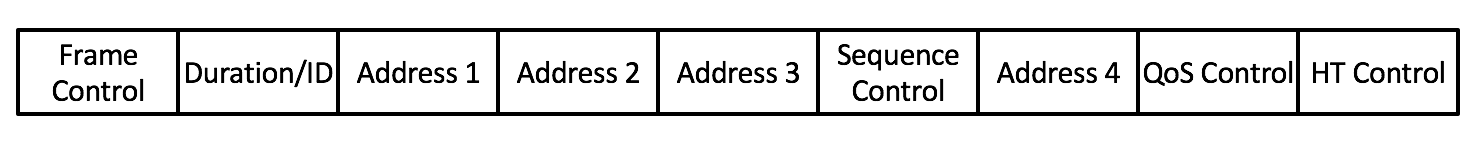
\includegraphics[width=\linewidth]{macHeader}}
			\caption{\ac{MPDU} format when using \ac{WPA}-2 \cite{802.11}}
			\label{fig:MpduFormat}
		\end{center}
		\vspace{-0.2 in}
	\end{figure}
}

\newcommand{\figMacHeader}{
	\begin{figure}[H]
		\begin{center}
			\makebox[\textwidth][c]{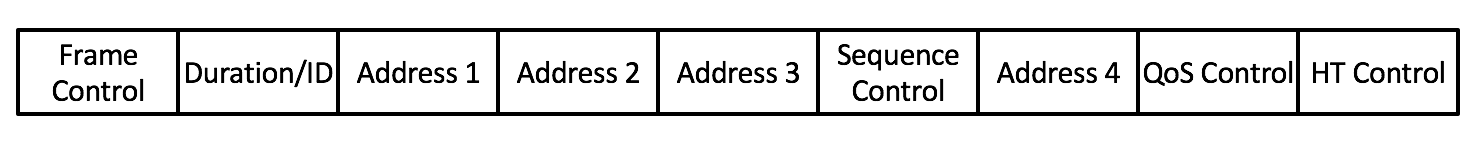
\includegraphics[width=\linewidth]{macHeader}}
			\caption{\ac{MAC} Header Frame Format \cite{802.11}}
			\label{fig:MacHeader}
		\end{center}
		\vspace{-0.2 in}
	\end{figure}
}

\newcommand{\figArchitecture}{\begin{figure}[H]
	\begin{center}
		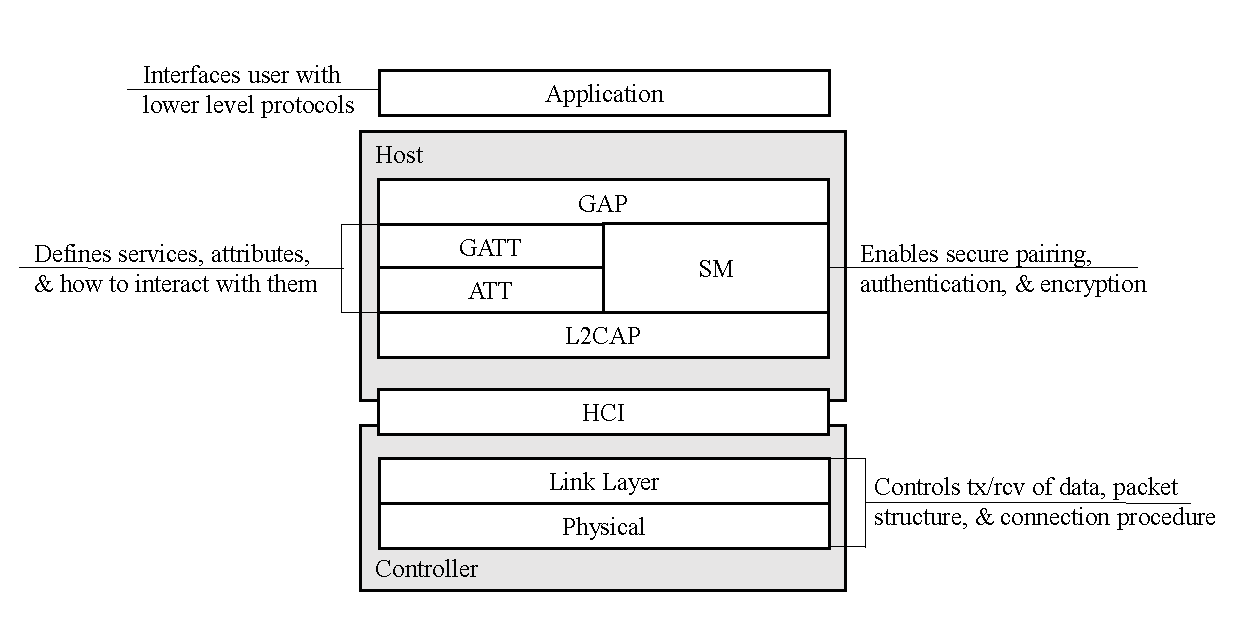
\includegraphics[width=4in]{architecture}
		\caption{The Bluetooth Low Energy Architecture}
		\label{fig:Architecture}
	\end{center}
	\vspace{-0.2 in}
\end{figure}
}

\newcommand{\figConnection}{\begin{figure}[H]
	\begin{center}
		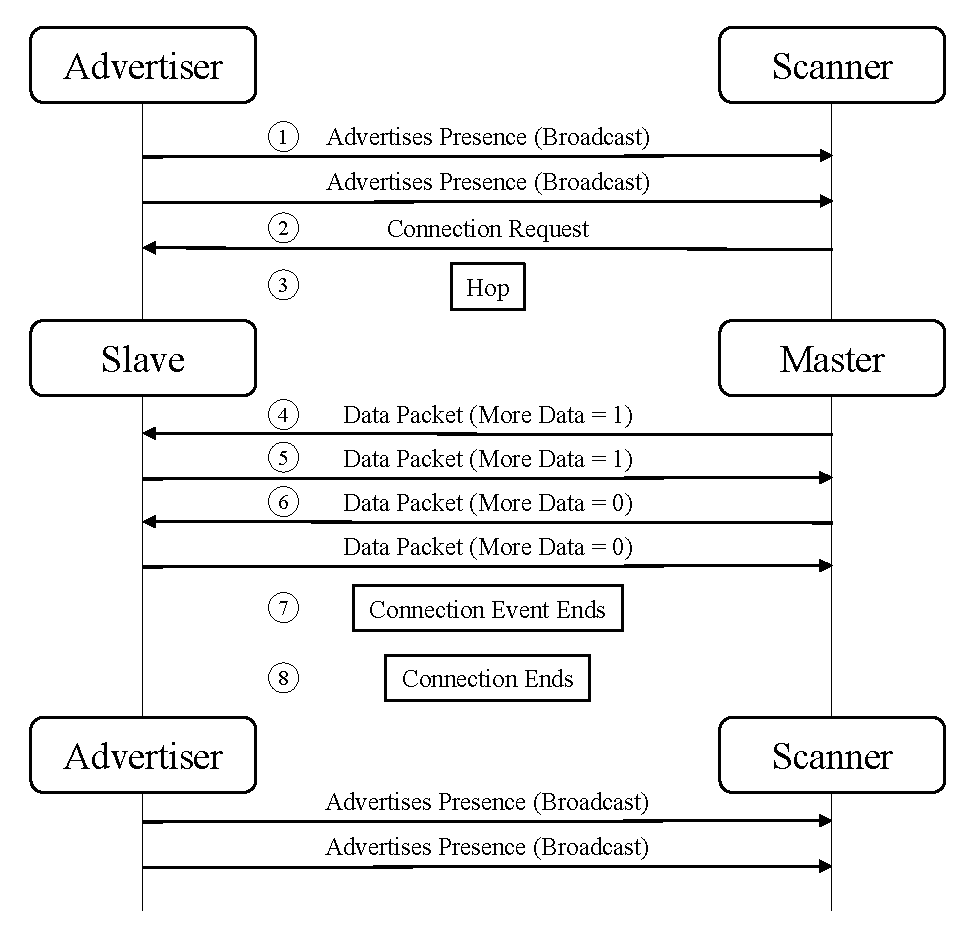
\includegraphics[width=4in]{connectionProcess}
		\caption{The \ac{BLE} Connection Process}
		\label{fig:Connection}
	\end{center}
	\vspace{-0.2 in}
\end{figure}
}

\newcommand{\figScanning}{\begin{figure}[H]
		\begin{center}
			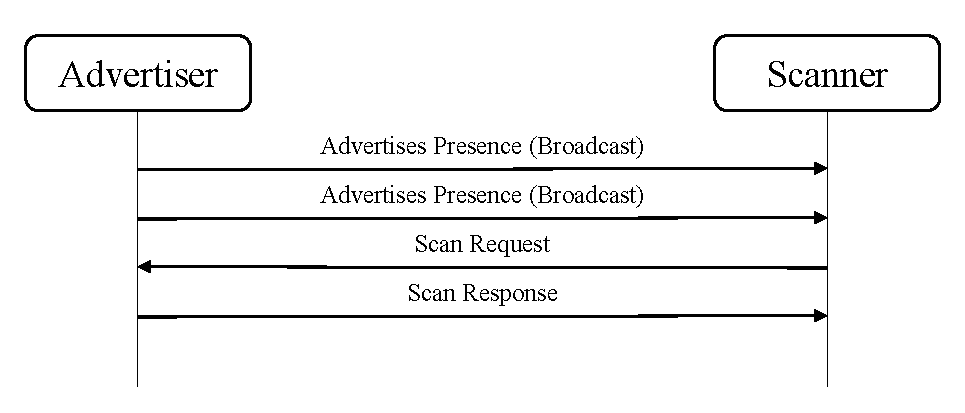
\includegraphics[width=4in]{activeScanning}
			\caption{Active Scanning Process}
			\label{fig:Scanning}
		\end{center}
		\vspace{-0.2 in}
	\end{figure}
}

\newcommand{\figChannel}{
	\begin{figure}[H]
		\begin{center}
			\includegraphics[width=5in]{channelMap}
			\caption{Bluetooth Low Energy channel mapping; darker channels represent advertisement channels}
			\label{fig:Channel}
		\end{center}
		\vspace{-0.2 in}
	\end{figure}
}

\newcommand{\figAccessPoint}{
	\begin{figure}[H]
		\begin{center}
			\makebox[\textwidth][c]{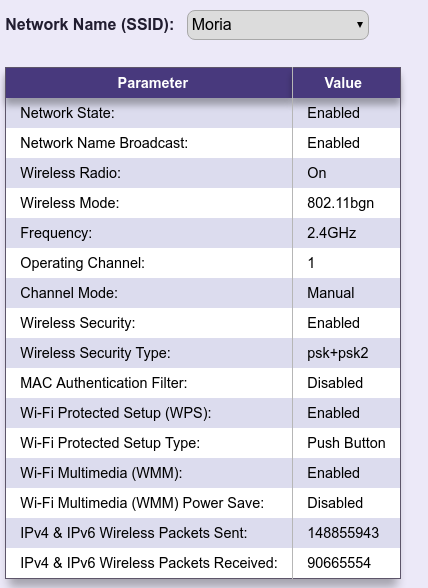
\includegraphics[width=2.5in]{accessPoint}}
			\caption{Prancing Pony Access Point Settings}
			\label{fig:AccessPoint}
		\end{center}
		\vspace{-0.2 in}
	\end{figure}
}

\newcommand{\figSystemDiagram}{
	\begin{figure}[h!]
		\begin{center}
			\centering
			\makebox[\textwidth][c]{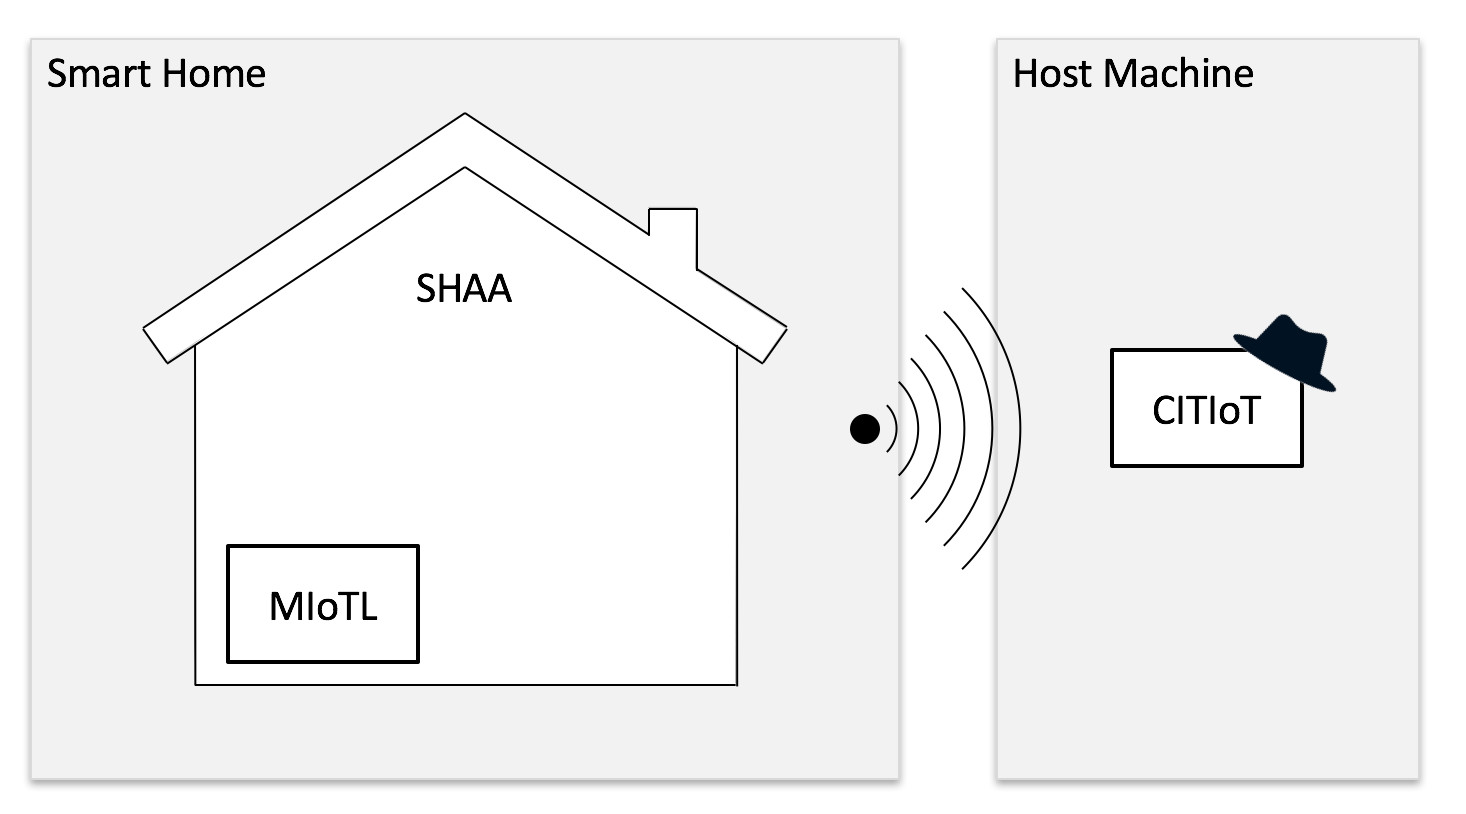
\includegraphics[width=4in]{systemDiagram}}
			\caption{Overall system diagram}
			\label{fig:SystemDiagram}
		\end{center}
		\vspace{-0.2 in}
	\end{figure}
}

\newcommand{\figShaaDiagram}{
	\begin{figure*}[h!]
		\begin{center}
			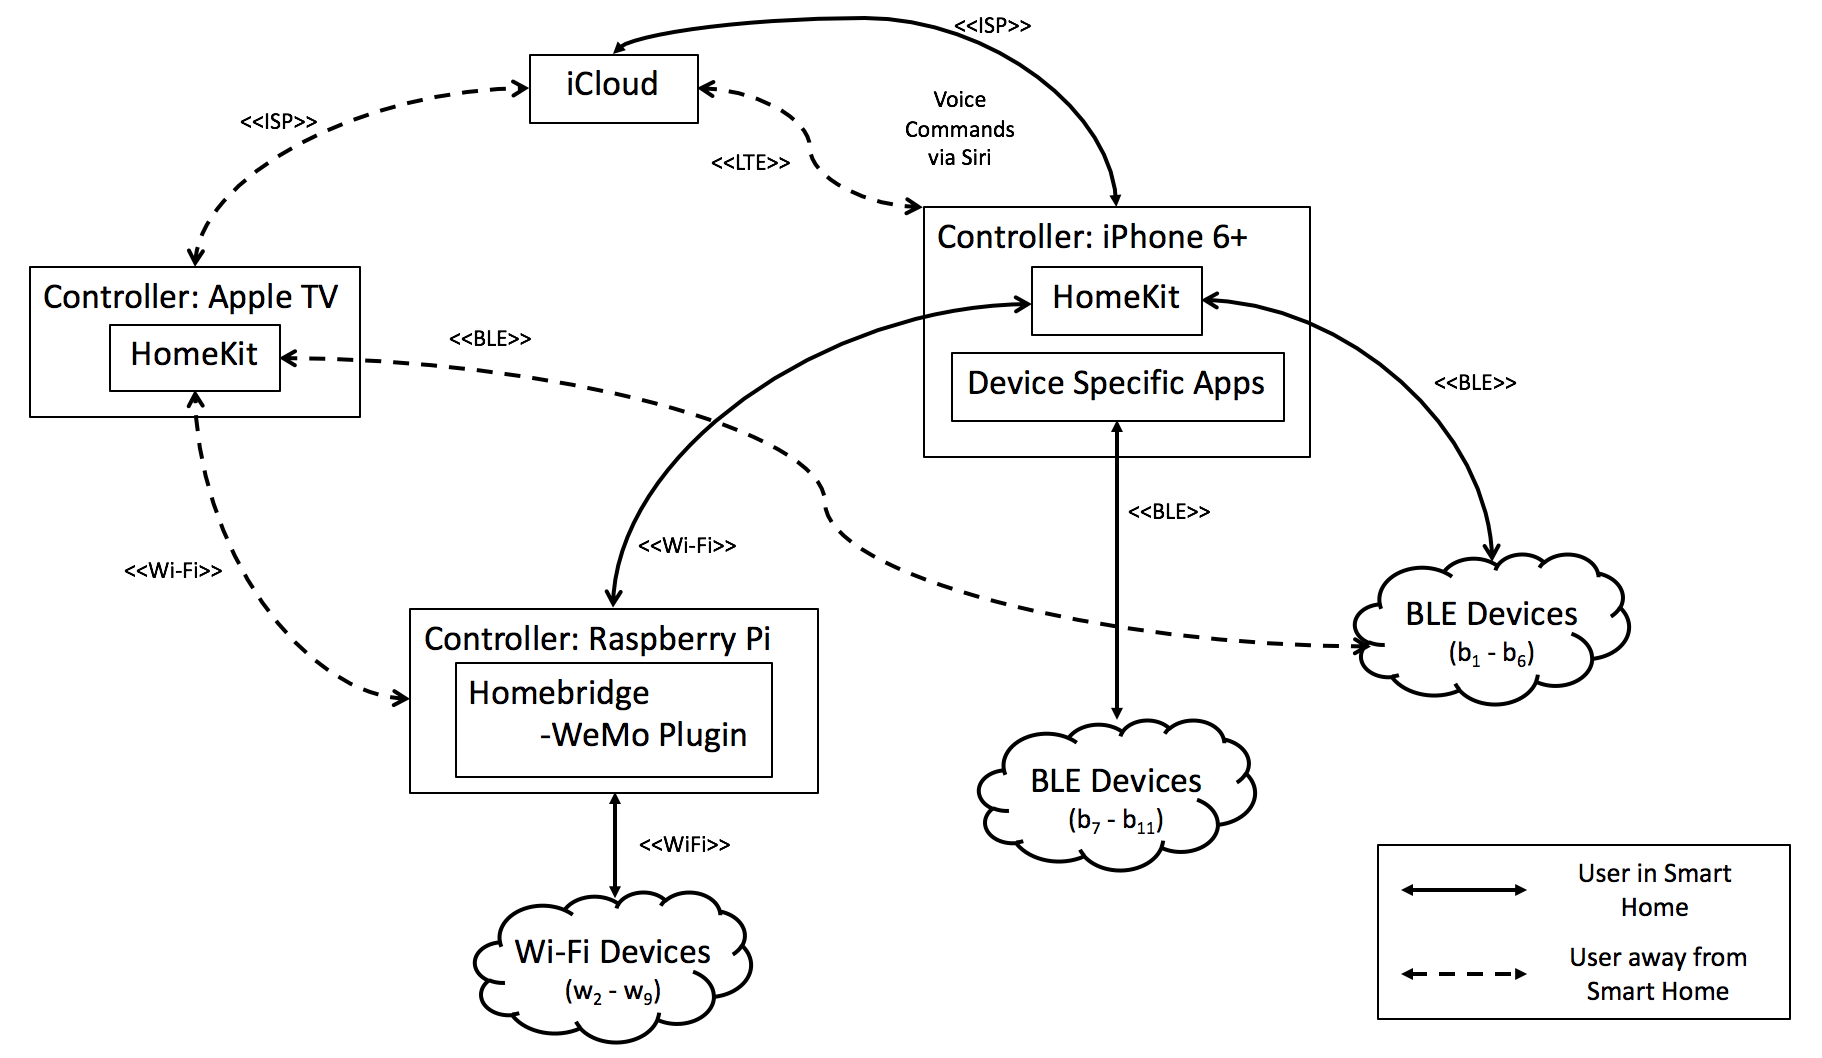
\includegraphics[width=\linewidth]{shaaDiagram}
			\caption{Diagram of SHAA components}
			\label{fig:ShaaDiagram}
		\end{center}
		\vspace{-0.2 in}
	\end{figure*}
}

\newcommand{\figCitiotDiagram}{
	\begin{figure*}[h!]
		\begin{center}
			\makebox[\textwidth][c]{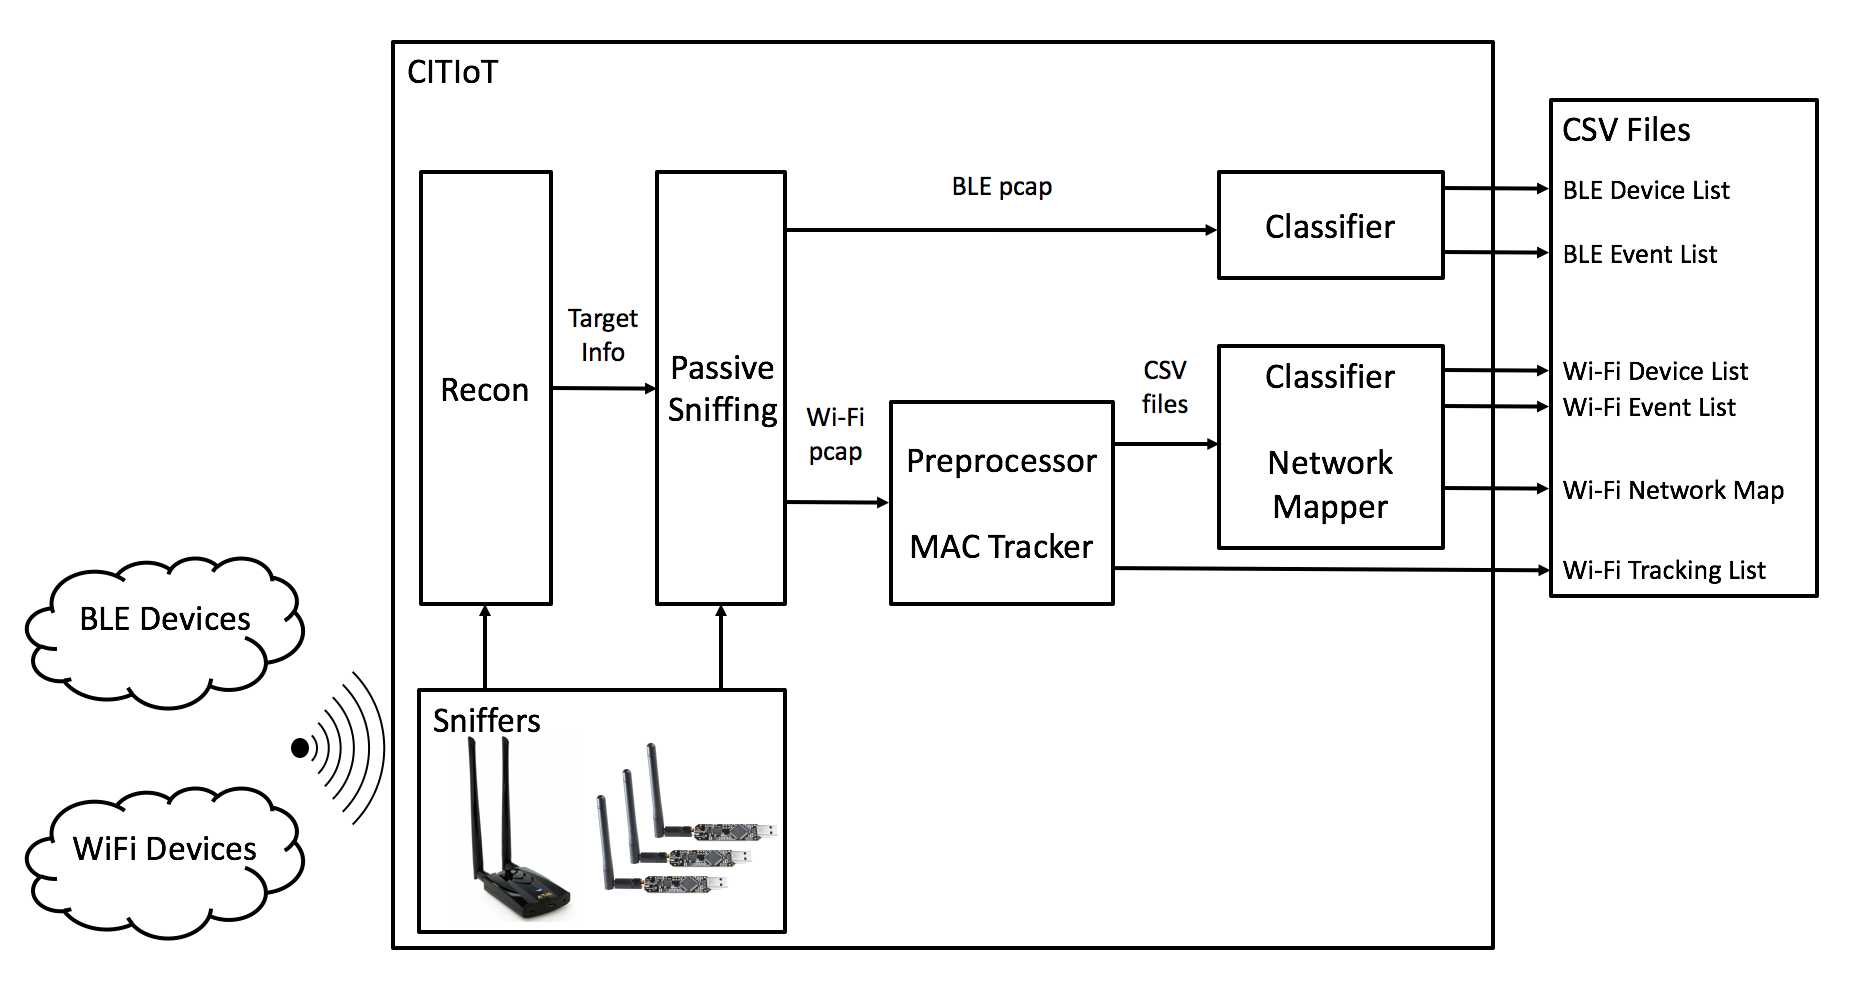
\includegraphics[width=\linewidth]{citiotDiagram}}
			\caption{Diagram of CITIoT tool components and interactions}
			\label{fig:CitiotDiagram}
		\end{center}
		\vspace{-0.2 in}
	\end{figure*}
}

\newcommand{\figReconScan}{
	\begin{figure*}[h!]
		\begin{center}
			\makebox[\textwidth][c]{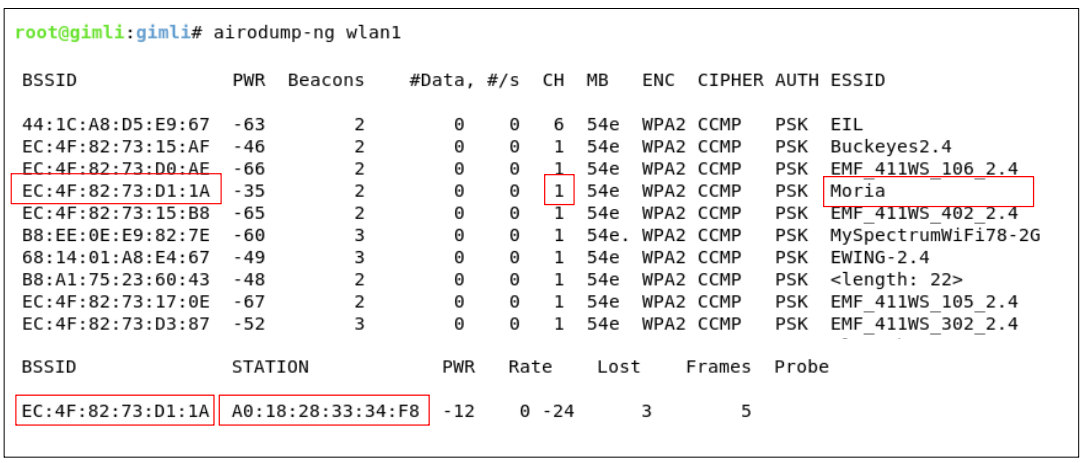
\includegraphics[width=\linewidth]{reconScan}}
			\caption{Command and results to accomplish a scan of Wi-Fi devices and associated \ac{AP}s}
			\label{fig:ReconScan}
		\end{center}
		\vspace{-0.2 in}
	\end{figure*}
}

\newcommand{\figScanDevices}{
	\begin{figure}[H]
		\begin{center}
			\makebox[\textwidth][c]{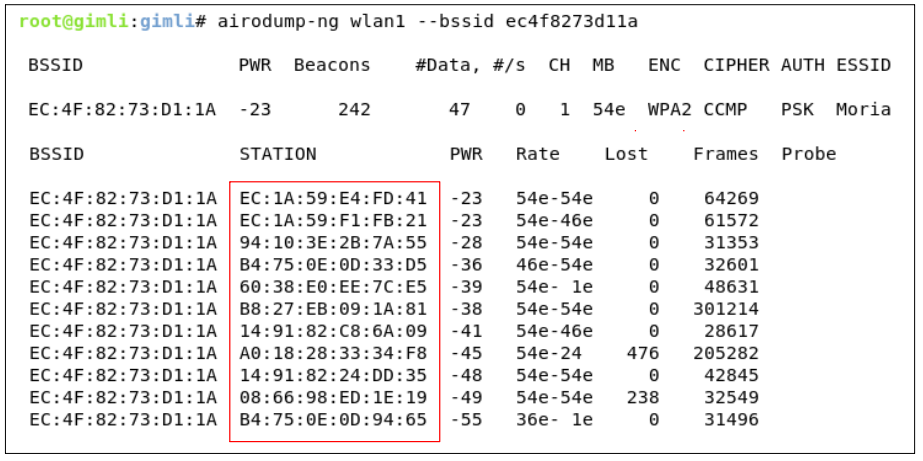
\includegraphics[width=\linewidth]{scanDevices}}
			\caption{Command and results to scan for devices connected to the target \ac{AP}}
			\label{fig:ScanDevices}
		\end{center}
		\vspace{-0.2 in}
	\end{figure}
}

\newcommand{\figOuiLookup}{
	\begin{figure}[H]
		\begin{center}
			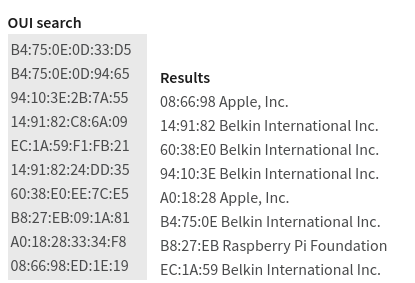
\includegraphics[width=3in]{ouiLookup}
			\caption{Wi-Fi MAC OUI search and results}
			\label{fig:OuiLookup}
		\end{center}
		\vspace{-0.2 in}
	\end{figure}
}

\newcommand{\figBleDeviceScan}{
	\begin{figure}[H]
		\begin{center}
			\makebox[\textwidth][c]{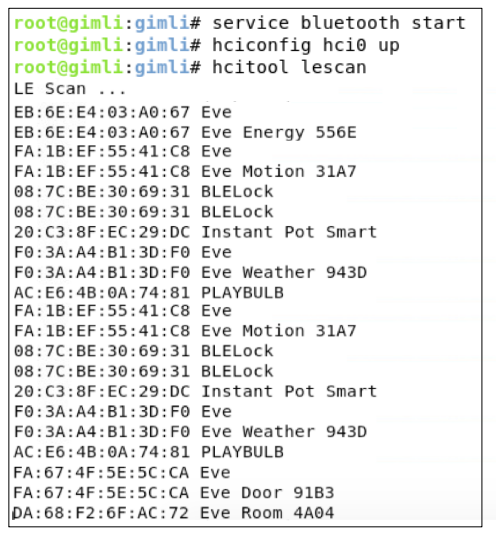
\includegraphics[width=3.5in]{bleDeviceScan}}
			\caption{Command and results to scan for \ac{BLE} devices within the smart home}
			\label{fig:BleDeviceScan}
		\end{center}
		\vspace{-0.2 in}
	\end{figure}
}

\newcommand{\figMonitorMode}{
	\begin{figure}[H]
		\begin{center}
			\makebox[\textwidth][c]{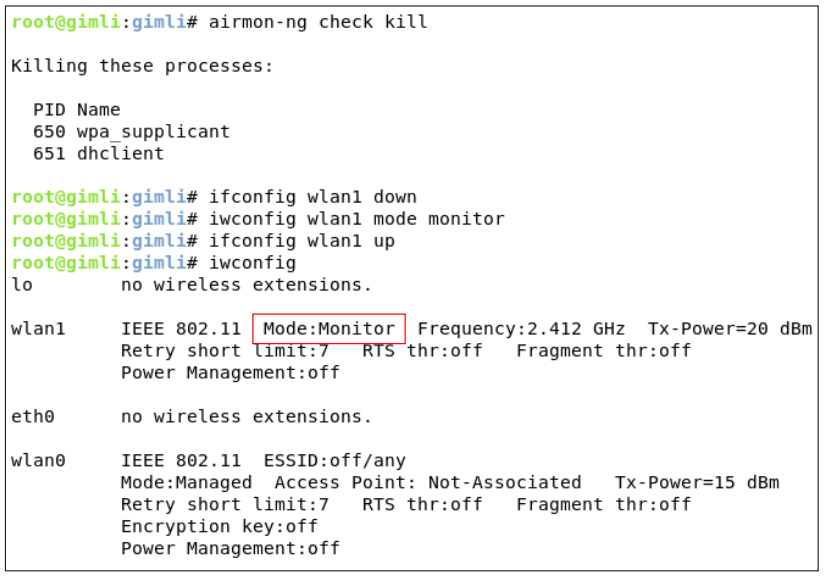
\includegraphics[width=\linewidth]{monitorMode}}
			\caption{Commands used to set Wi-Fi interface to monitor mode}
			\label{fig:MonitorMode}
		\end{center}
		\vspace{-0.2 in}
	\end{figure}
}

\newcommand{\figWifiCaptCmd}{
	\begin{figure}[H]
		\begin{center}
			\makebox[\textwidth][c]{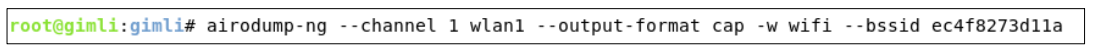
\includegraphics[height=.75cm]{wifiCaptCmd}}
			\caption{Command and options used to capture Wi-Fi traffic}
			\label{fig:WifiCaptCmd}
		\end{center}
		\vspace{-0.2 in}
	\end{figure}
}

\newcommand{\figBleCaptCmd}{
	\begin{figure}[H]
		\begin{center}
			\makebox[\textwidth][c]{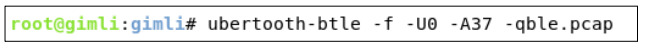
\includegraphics[height=.75cm]{bleCaptCmd}}
			\caption{Example command and options used to capture \ac{BLE} traffic}
			\label{fig:BleCaptCmd}
		\end{center}
		\vspace{-0.2 in}
	\end{figure}
}

\newcommand{\figCorruptTimePacket}{
	\begin{figure}[H]
		\begin{center}
			\makebox[\textwidth][c]{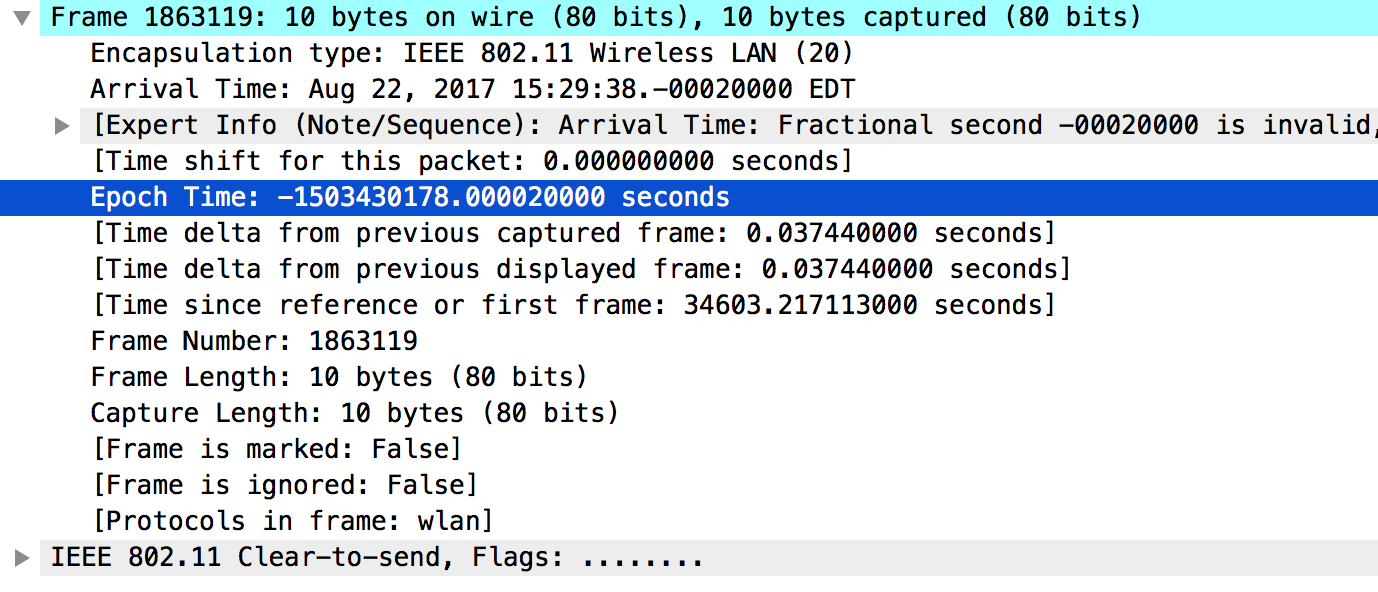
\includegraphics[width=\linewidth]{corruptTimePacket}}
			\caption{Encrypted packet used in \ac{MAC} tracker showing corrupted timestamp}
			\label{fig:CorruptTimePacket}
		\end{center}
		\vspace{-0.2 in}
	\end{figure}
}

\newcommand{\figWrongFrameNumber}{
	\begin{figure}[H]
		\begin{center}
			\makebox[\textwidth][c]{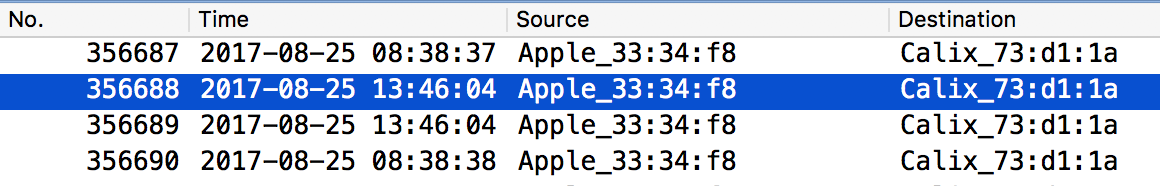
\includegraphics[width=\linewidth]{wrongFrameNumber}}
			\caption{Encrypted packets used in \ac{MAC} tracker showing sequential frame numbers but wrong times}
			\label{fig:WrongFrameNumber}
		\end{center}
		\vspace{-0.2 in}
	\end{figure}
}

\newcommand{\figTrainingToDevice}{
	\begin{figure}[H]
		\centering
		\begin{subfigure}{.485\textwidth}
			\centering
			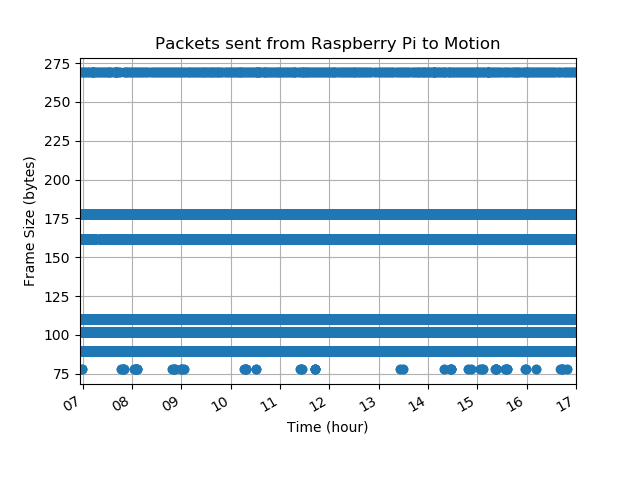
\includegraphics[width=\linewidth]{trngToMotion}
			\caption{}
		\end{subfigure}%
		\begin{subfigure}{.485\textwidth}
			\centering
			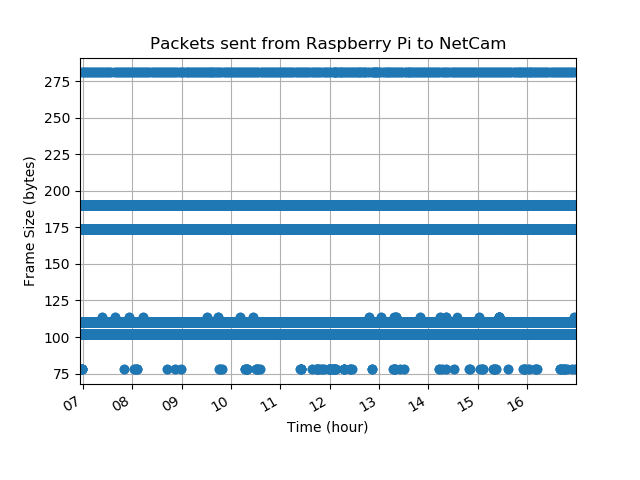
\includegraphics[width=\linewidth]{trngToNetcam}
			\caption{}
		\end{subfigure}
		\begin{subfigure}{.485\textwidth}
			\centering
			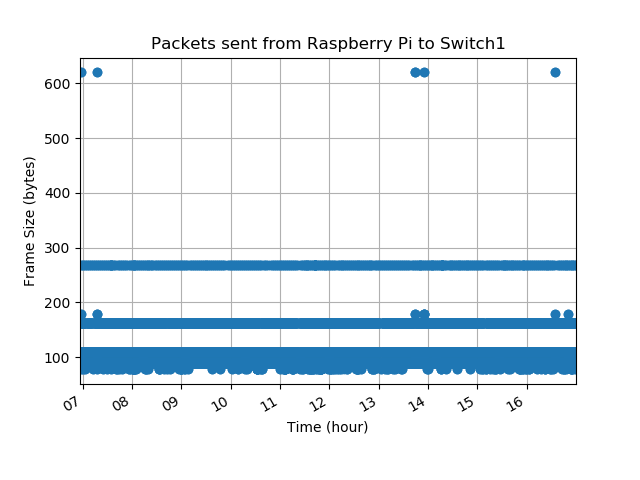
\includegraphics[width=\linewidth]{trngToSwitch1}
			\caption{}
		\end{subfigure}%
		\begin{subfigure}{.485\textwidth}
			\centering
			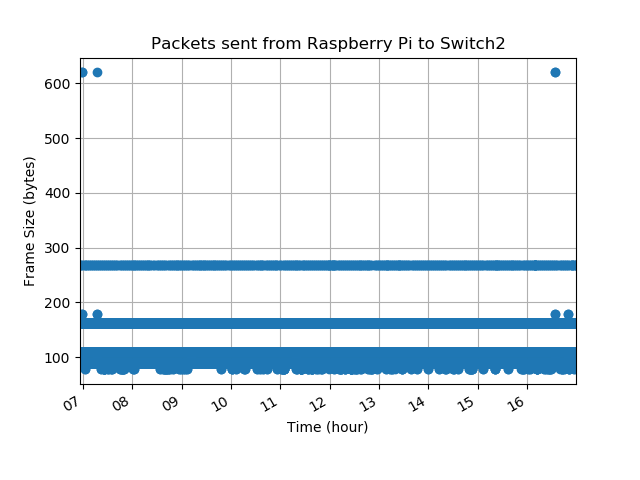
\includegraphics[width=\linewidth]{trngToSwitch2}
			\caption{}
		\end{subfigure}
		\begin{subfigure}{.485\textwidth}
			\centering
			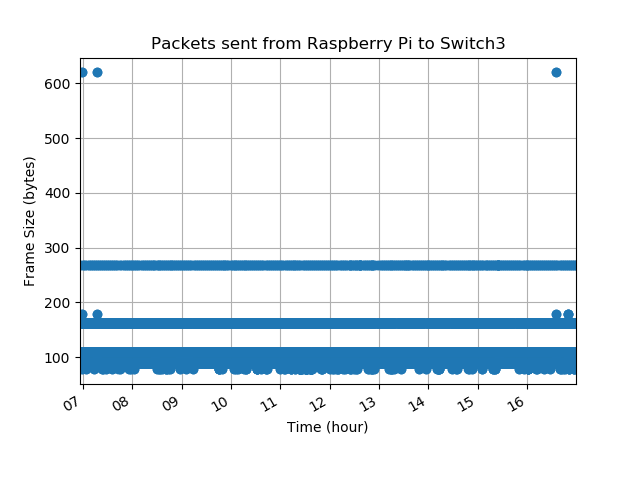
\includegraphics[width=\linewidth]{trngToSwitch3}
			\caption{}
		\end{subfigure}%
		\begin{subfigure}{.485\textwidth}
			\centering
			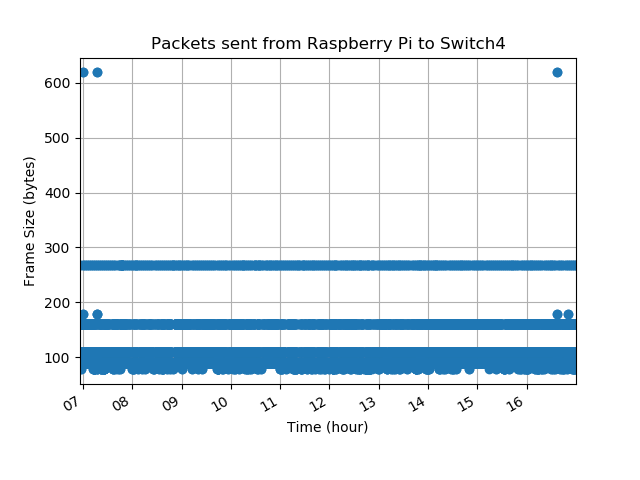
\includegraphics[width=\linewidth]{trngToSwitch4}
			\caption{}
		\end{subfigure}
		\begin{subfigure}{.485\textwidth}
			\centering
			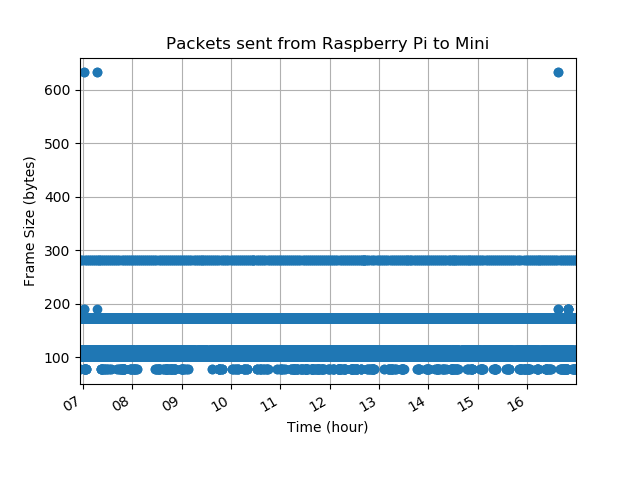
\includegraphics[width=\linewidth]{trngToMini}
			\caption{}
		\end{subfigure}%
		\begin{subfigure}{.485\textwidth}
			\centering
			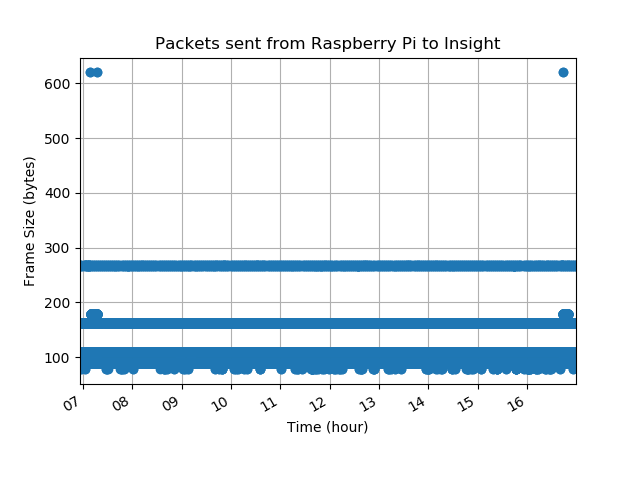
\includegraphics[width=\linewidth]{trngToInsight}
			\caption{}
		\end{subfigure}
		\caption{Training plots of packets sent from raspberry pi to device}
		\label{fig:TrainingToDevice}
	\end{figure}
}

\newcommand{\figTrainingFromDevice}{
	\begin{figure}[H]
		\centering
		\begin{subfigure}{.485\textwidth}
			\centering
			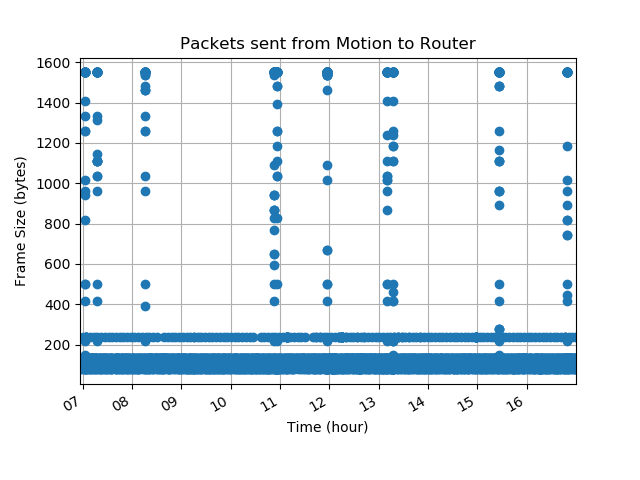
\includegraphics[width=\linewidth]{trngFromMotion}
			\caption{}
		\end{subfigure}%
		\begin{subfigure}{.485\textwidth}
			\centering
			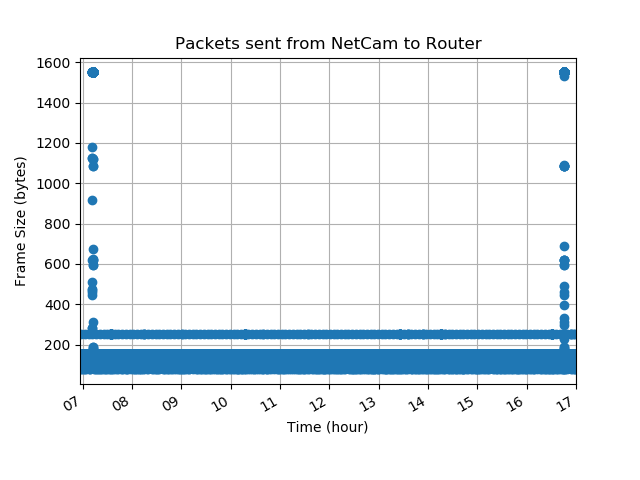
\includegraphics[width=\linewidth]{trngFromNetcam}
			\caption{}
		\end{subfigure}
		\begin{subfigure}{.485\textwidth}
			\centering
			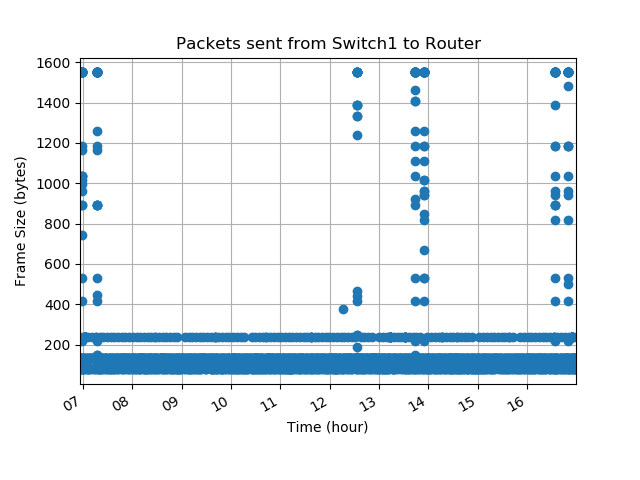
\includegraphics[width=\linewidth]{trngFromSwitch1}
			\caption{}
		\end{subfigure}%
		\begin{subfigure}{.485\textwidth}
			\centering
			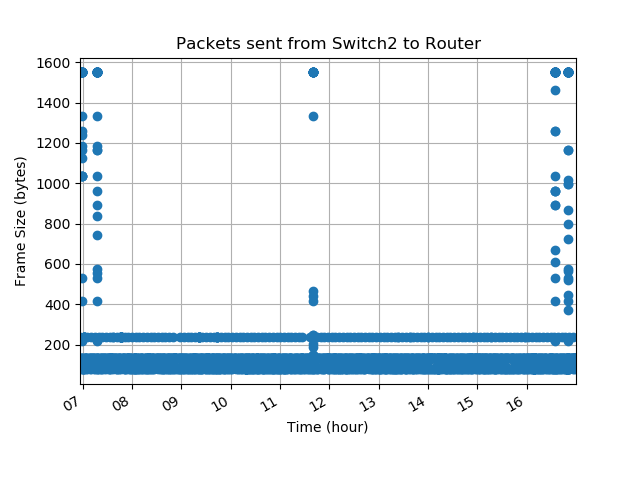
\includegraphics[width=\linewidth]{trngFromSwitch2}
			\caption{}
		\end{subfigure}
		\begin{subfigure}{.485\textwidth}
			\centering
			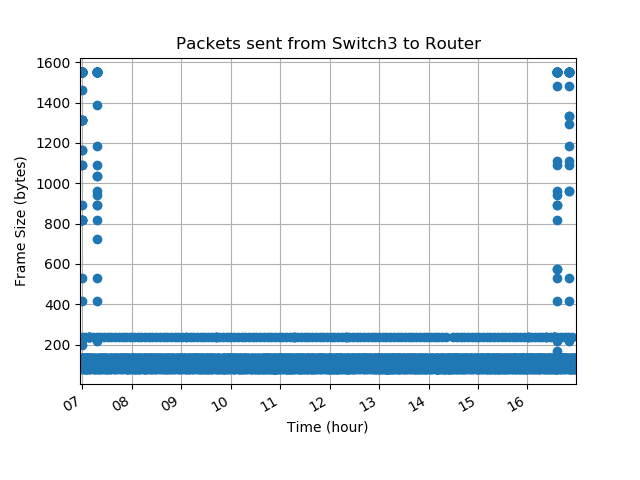
\includegraphics[width=\linewidth]{trngFromSwitch3}
			\caption{}
		\end{subfigure}%
		\begin{subfigure}{.485\textwidth}
			\centering
			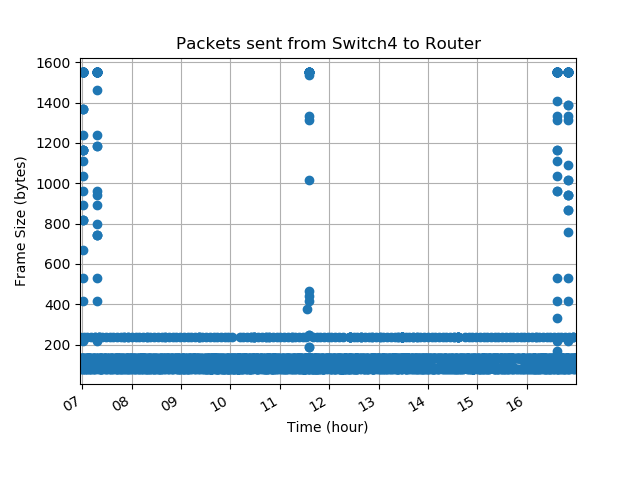
\includegraphics[width=\linewidth]{trngFromSwitch4}
			\caption{}
		\end{subfigure}
		\begin{subfigure}{.485\textwidth}
			\centering
			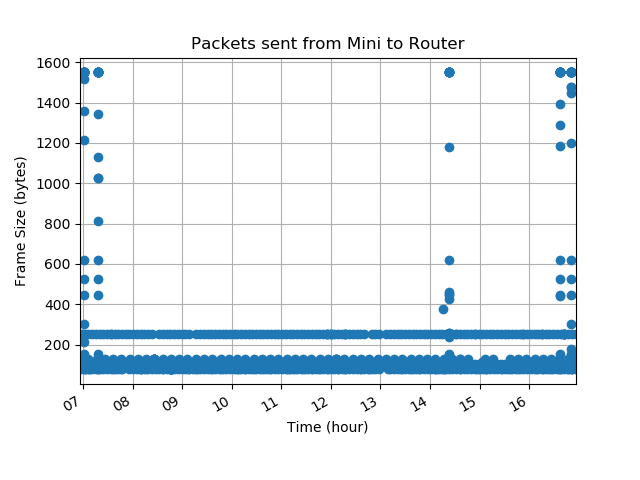
\includegraphics[width=\linewidth]{trngFromMini}
			\caption{}
		\end{subfigure}%
		\begin{subfigure}{.485\textwidth}
			\centering
			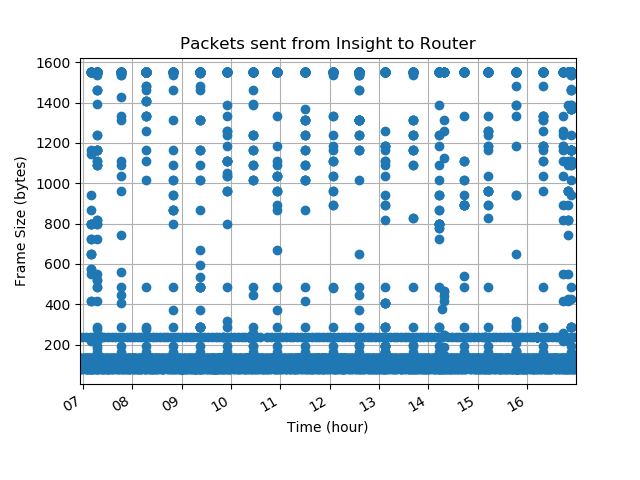
\includegraphics[width=\linewidth]{trngFromInsight}
			\caption{}
		\end{subfigure}
		\caption{Training plots of packets sent from device to the router}
		\label{fig:TrainingFromDevice}
	\end{figure}
}

\newcommand{\figClassificationToNetcam}{
	\begin{figure}[H]
		\begin{center}
			\makebox[\textwidth][c]{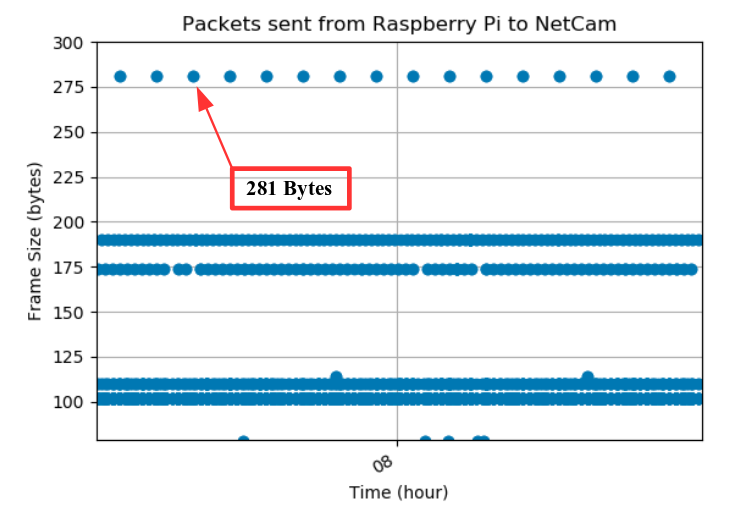
\includegraphics[width=5in]{classificationToNetcam}}
			\caption{Figure~\ref{fig:TrainingToDevice}(b) zoomed in on unique packet traffic used to classify camera devices}
			\label{fig:ClassificationToNetcam}
		\end{center}
		\vspace{-0.2 in}
	\end{figure}
}

\newcommand{\figClassificationToMotion}{
	\begin{figure}[H]
		\begin{center}
			\makebox[\textwidth][c]{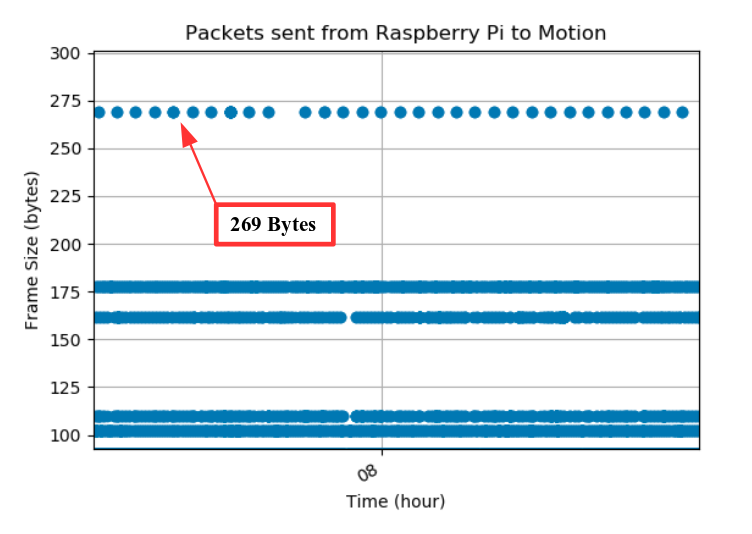
\includegraphics[width=5in]{classificationToMotion}}
			\caption{Figure~\ref{fig:TrainingToDevice}(a) zoomed in on unique packet traffic used to classify motion devices}
			\label{fig:ClassificationToMotion}
		\end{center}
		\vspace{-0.2 in}
	\end{figure}
}

\newcommand{\figClassificationToSwitch}{
	\begin{figure}[H]
		\begin{center}
			\makebox[\textwidth][c]{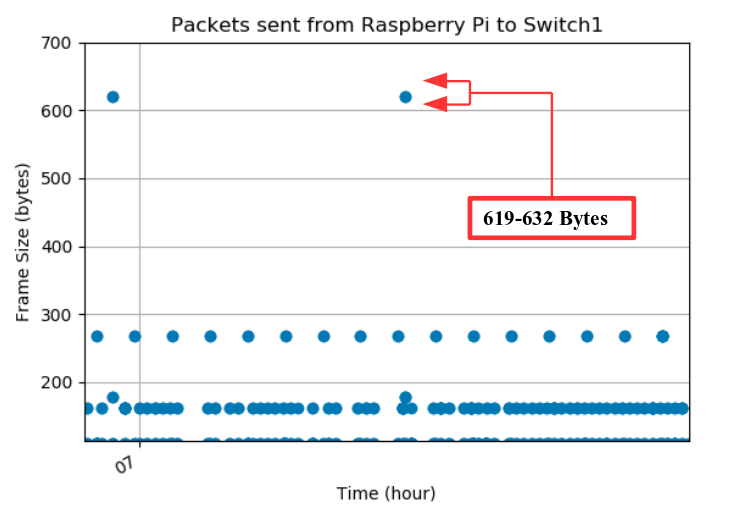
\includegraphics[width=5in]{classificationToSwitch}}
			\caption{Figure~\ref{fig:TrainingToDevice}(c) zoomed in on unique packet traffic used to classify outlet devices}
			\label{fig:ClassificationToSwitch}
		\end{center}
		\vspace{-0.2 in}
	\end{figure}
}

\newcommand{\figDeviceClassification}{
	\begin{figure}[H]
		\begin{center}
			\makebox[\textwidth][c]{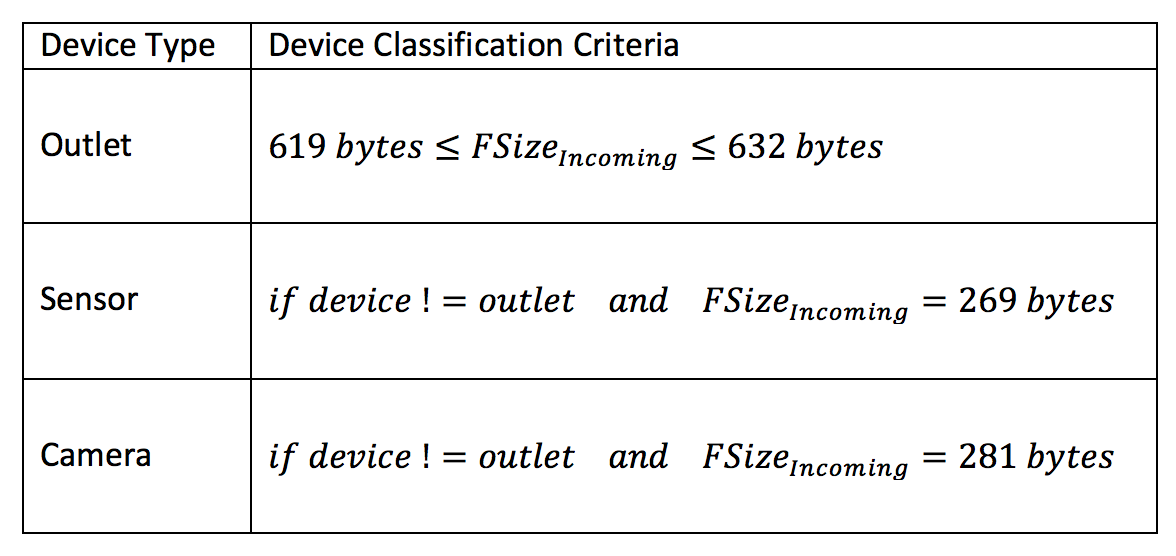
\includegraphics[height=2in]{deviceClassification}}
			\caption{Criteria used to classify devices}
			\label{fig:DeviceClassification}
		\end{center}
		\vspace{-0.2 in}
	\end{figure}
}

\newcommand{\figIdentificationToMini}{
	\begin{figure}[H]
		\begin{center}
			\makebox[\textwidth][c]{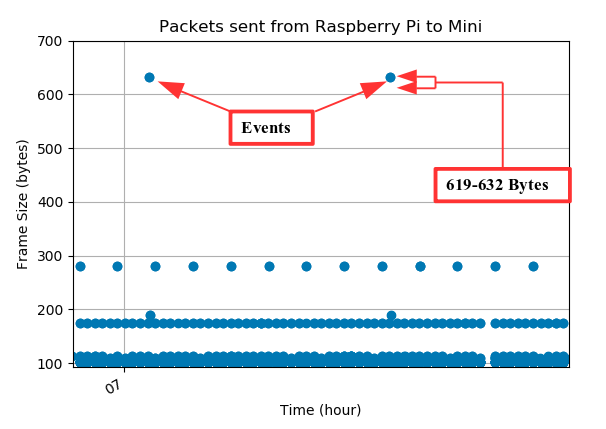
\includegraphics[width=5in]{identificationToMini}}
			\caption{Figure~\ref{fig:TrainingToDevice}(g) zoomed in on unique packet traffic used to identify outlet events}
			\label{fig:IdentificationToMini}
		\end{center}
		\vspace{-0.2 in}
	\end{figure}
}

\newcommand{\figIdentificationFromNetcam}{
	\begin{figure}[H]
		\begin{center}
			\makebox[\textwidth][c]{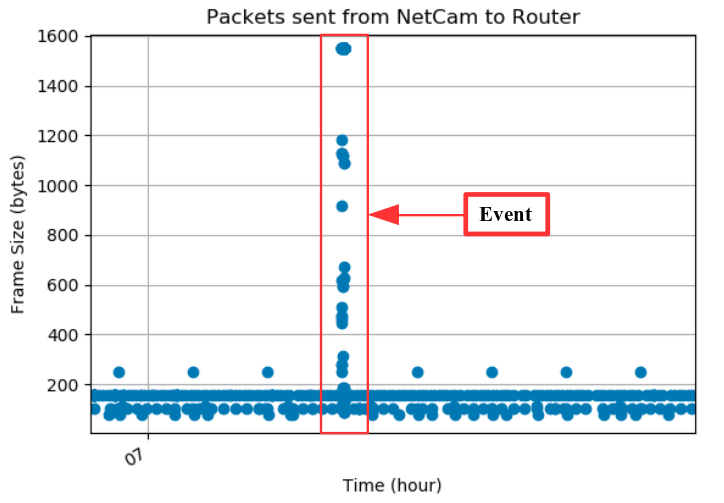
\includegraphics[width=5in]{identificationFromNetcam}}
			\caption{Figure~\ref{fig:TrainingFromDevice}(b) zoomed in on unique packet traffic used to identify camera events}
			\label{fig:IdentificationFromNetcam}
		\end{center}
		\vspace{-0.2 in}
	\end{figure}
}

\newcommand{\figIdentificationFromNetcamCum}{
	\begin{figure}[H]
		\begin{center}
			\makebox[\textwidth][c]{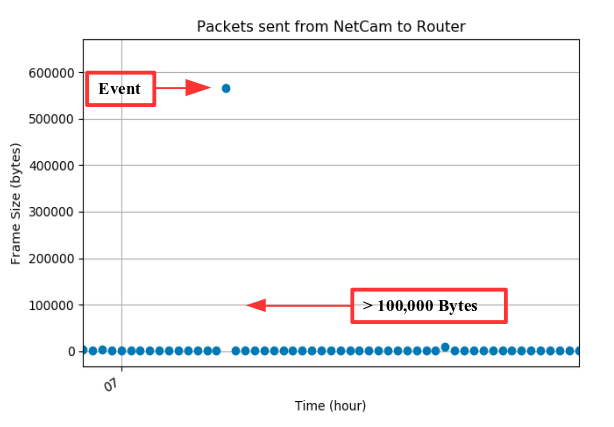
\includegraphics[width=5in]{identificationFromNetcamCum}}
			\caption{Figure~\ref{fig:TrainingFromDevice}(b) with one minute cumulative frame size zoomed in on unique packet traffic used to identify camera events}
			\label{fig:IdentificationFromNetcamCum}
		\end{center}
		\vspace{-0.2 in}
	\end{figure}
}

\newcommand{\figIdentificationFromMotion}{
	\begin{figure}[H]
		\begin{center}
			\makebox[\textwidth][c]{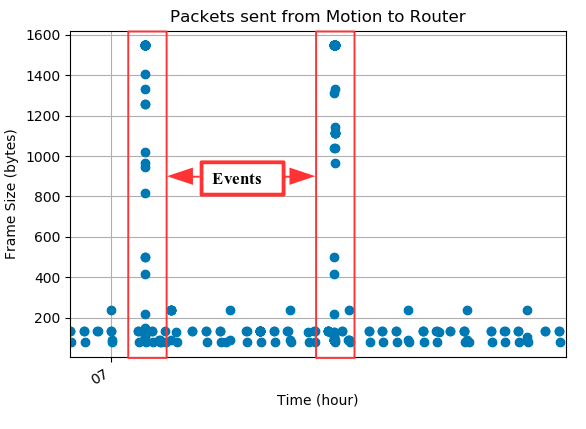
\includegraphics[width=5in]{identificationFromMotion}}
			\caption{Figure~\ref{fig:TrainingFromDevice}(a) zoomed in on unique packet traffic used to identify motion events}
			\label{fig:IdentificationFromMotion}
		\end{center}
		\vspace{-0.2 in}
	\end{figure}
}

\newcommand{\figIdentificationFromMotionCum}{
	\begin{figure}[H]
		\begin{center}
			\makebox[\textwidth][c]{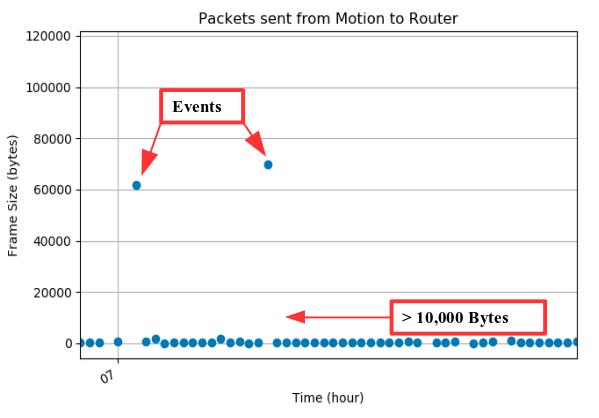
\includegraphics[width=5in]{identificationFromMotionCum}}
			\caption{Figure~\ref{fig:TrainingFromDevice}(a) with one minute cumulative frame size zoomed in on unique packet traffic used to identify motion events}
			\label{fig:IdentificationFromMotionCum}
		\end{center}
		\vspace{-0.2 in}
	\end{figure}
}

\newcommand{\figEventIdentification}{
	\begin{figure}[H]
		\begin{center}
			\makebox[\textwidth][c]{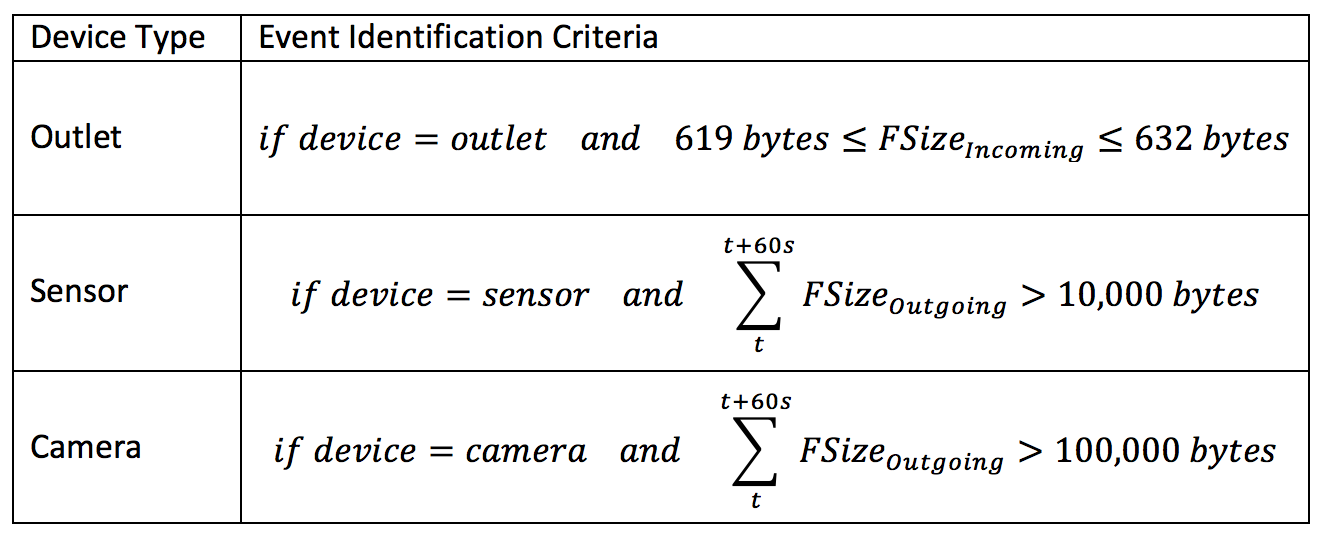
\includegraphics[height=2in]{eventIdentification}}
			\caption{Criteria used to identify events}
			\label{fig:EventIdentification}
		\end{center}
		\vspace{-0.2 in}
	\end{figure}
}

\newcommand{\figSubscribePacket}{
	\begin{figure}[H]
		\begin{center}
			\makebox[\textwidth][c]{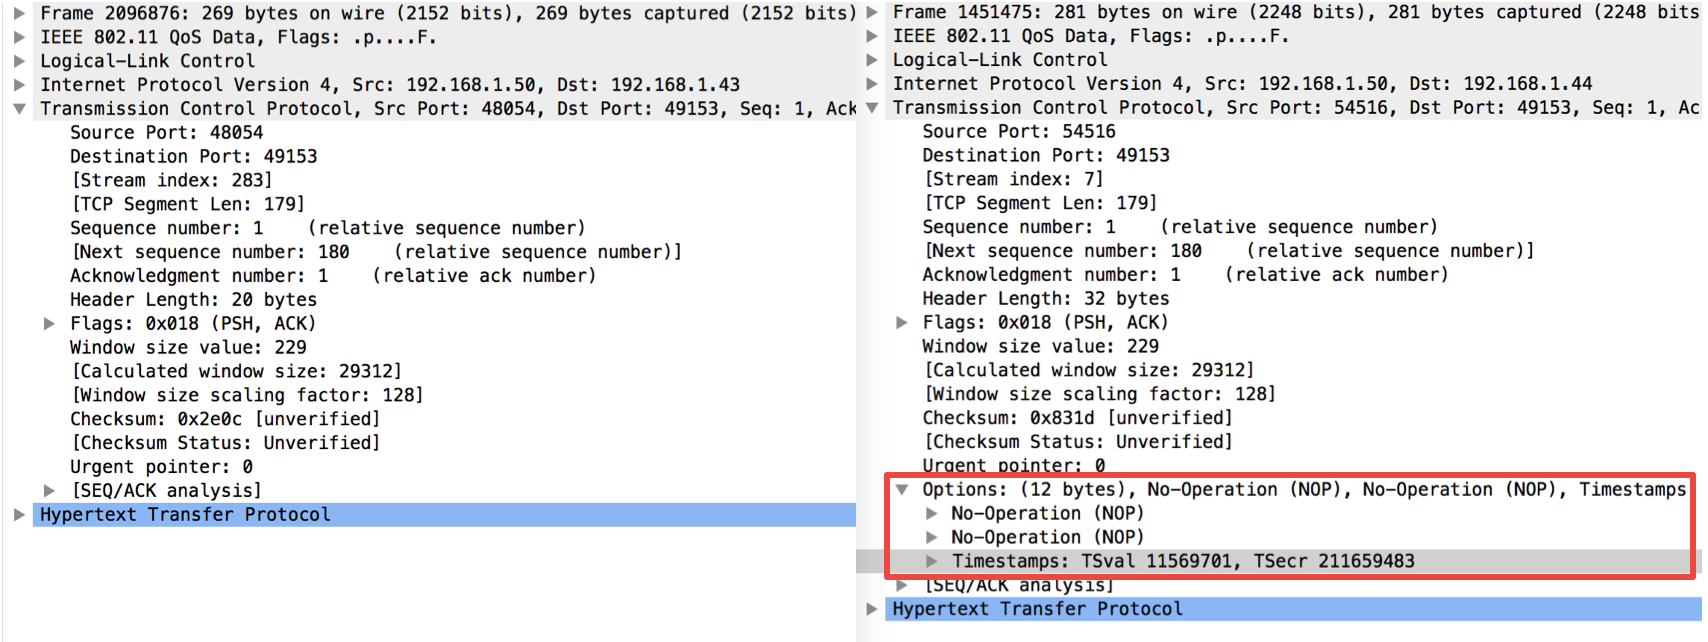
\includegraphics[width=\linewidth]{subscribePacket}}
			\caption{Decrypted \texttt{SUBSCRIBE} packets from Raspberry Pi to the NetCam and Motion devices depicting difference in frame length}
			\label{fig:SubscribePacket}
		\end{center}
		\vspace{-0.2 in}
	\end{figure}
}

\newcommand{\figPostPacket}{
	\begin{figure}[H]
		\begin{center}
			\makebox[\textwidth][c]{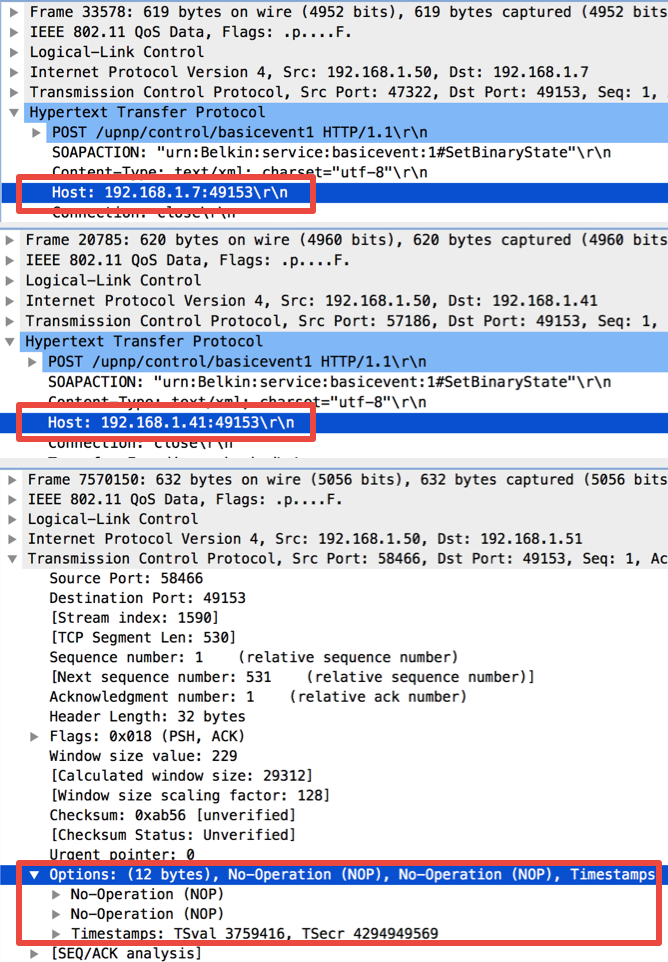
\includegraphics[width=.975\linewidth]{postPacket}}
			\caption{Decrypted \texttt{POST} packets from Raspberry Pi to the Switch4, Switch2, and Mini depicting differences in frame length}
			\label{fig:PostPacket}
		\end{center}
		\vspace{-0.2 in}
	\end{figure}
}

\newcommand{\figNetworkMap}{
	\begin{figure}[H]
		\begin{center}
			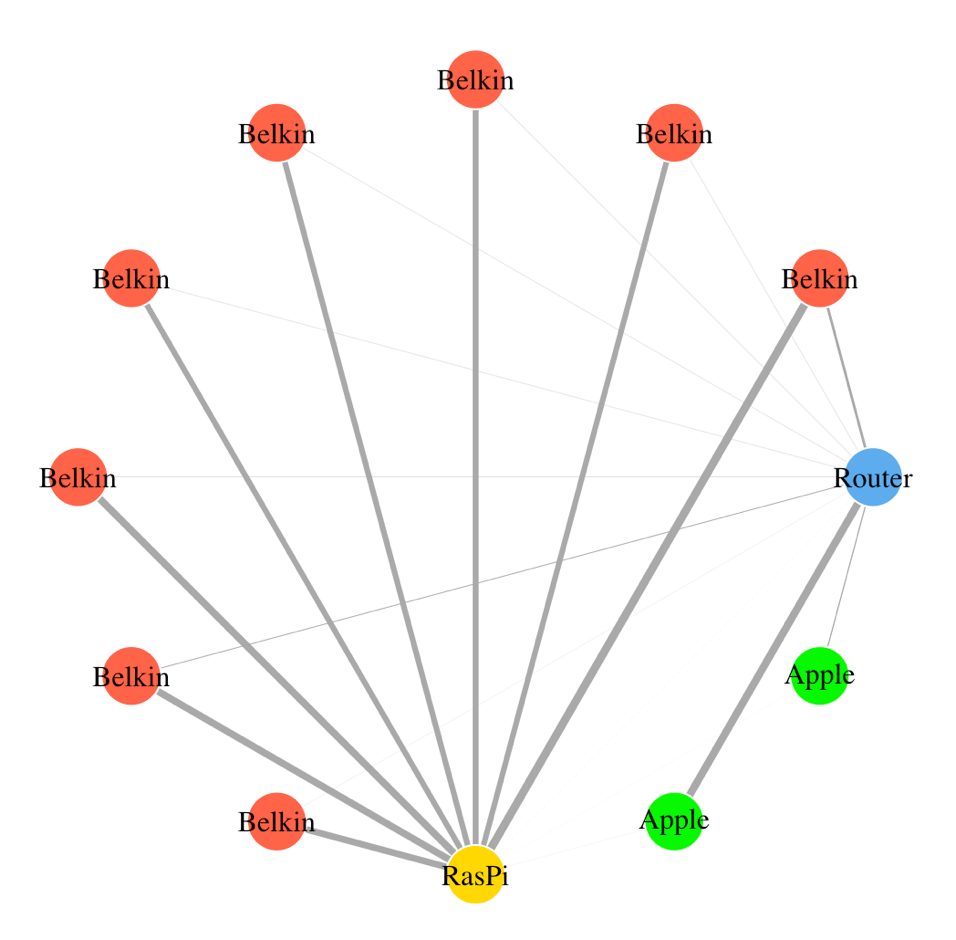
\includegraphics[width=5in]{networkMap}
			\caption{Network mapping of smart home architecture}
			\label{fig:NetworkMap}
		\end{center}
		\vspace{-0.2 in}
	\end{figure}
}

\newcommand{\figMiotlDiagram}{
	\begin{figure*}[h!]
		\begin{center}
			\includegraphics[width=3in]{miotlDiagram}
			\caption{Diagram of MIoTL tool components}
			\label{fig:MiotlDiagram}
		\end{center}
		\vspace{-0.2 in}
	\end{figure*}
}

\newcommand{\figSutCutDiagram}{
	\begin{figure*}[h!]
		\begin{center}
			\includegraphics[width=\linewidth]{sutCutDiagram}
			\caption{System Under Test (SUT) and Component Under Test (CUT) diagram}
			\label{fig:SutCutDiagram}
		\end{center}
		\vspace{-0.2 in}
	\end{figure*}
}

\newcommand{\figShaaExperimentDiagram}{
	\begin{figure*}[h!]
		\begin{center}
			\includegraphics[width=\linewidth]{shaaExperimentDiagram}
			\caption{Approximate layout of devices within \ac{SHAA} for experimentation (not to scale)}
			\label{fig:ShaaExperimentDiagram}
		\end{center}
		\vspace{-0.2 in}
	\end{figure*}
}

\newcommand{\figSnifferExperimentSetup}{
	\begin{figure*}[h!]
		\begin{center}
			\includegraphics[width=\linewidth]{snifferExperimentSetup}
			\caption{Layout of sniffer antennae for experimentation}
			\label{fig:SnifferExperimentSetup}
		\end{center}
		\vspace{-0.2 in}
	\end{figure*}
}

\newcommand{\figDataCollectionFramework}{
	\begin{figure}[h!]
		\begin{center}
			\includegraphics[width=\linewidth, height = 5cm]{hostMachine}
			\caption{Data Collection Framework}
			\label{fig:DataCollectionFramework}
		\end{center}
		\vspace{-0.2 in}
	\end{figure}
}

\newcommand{\figSampleResults}{
\begin{figure}[H]
	\begin{center}
		\includegraphics[width=\linewidth]{sampleResults}
		\caption{Example graph comparing CITIoT events with actual events}
		\label{fig:SampleResults}
	\end{center}
	\vspace{-0.2 in}
\end{figure}
}

\newcommand{\figCitiot}{
	\begin{figure}[H]
		\begin{center}
			\makebox[\textwidth][c]{\includegraphics[width=5in]{citiot}}
			\caption{CITIoT Architecture}
			\label{fig:Citiot}
		\end{center}
		\vspace{-0.2 in}
	\end{figure}
}

\newcommand{\figReconScanning}{
	\begin{figure}[H]
		\begin{center}
			\makebox[\textwidth][c]{\includegraphics[width=5in]{reconScanning}}
			\caption{Scanning command along with output.}
			\label{fig:ReconScanning}
		\end{center}
		\vspace{-0.2 in}
	\end{figure}
}

\newcommand{\figNetworkMapping}{
	\begin{figure}[tbp]
		\begin{center}
			\includegraphics[width=3in, height=7cm]{networkMapping}
			\caption{Network mapping of smart home architecture; thicker lines mean stronger correlation between devices.}
			\label{fig:NetworkMapping}
		\end{center}
		\vspace{-0.2 in}
	\end{figure}
}

\newcommand{\figMethodologyOverview}{
	\begin{figure}[H]
		\begin{center}
			\makebox[\textwidth][c]{\includegraphics[width=6in]{methodologyOverview}}
			\caption{Overall scenario setup.}
			\label{fig:MethodologyOverview}
		\end{center}
		\vspace{-0.2 in}
	\end{figure}
}

\newcommand{\figDeviceId}{
	\begin{figure}[H]
	\centering
		\begin{minipage}{.5\textwidth}
			\centering
			\includegraphics[width=1\linewidth]{deviceIdOutlet}
			\caption{Outlet device.}
			\label{fig:DeviceIdOutlet}
		\end{minipage}%
		\begin{minipage}{.5\textwidth}
			\centering
			\includegraphics[width=1\linewidth]{deviceIdSensor}
			\caption{Sensor device.}
			\label{fig:DeviceIdSensor}
		\end{minipage}
		\begin{minipage}{.5\textwidth}
			\centering
			\includegraphics[width=1\linewidth]{deviceIdCamera}
			\caption{Camera device.}
			\label{fig:DeviceIdCamera}
		\end{minipage}
	\end{figure}
}


\newcommand{\figExamplePlotOne}{
	\begin{figure}[H]
		\begin{center}
			\makebox[\textwidth][c]{\includegraphics[width=4.5in]{examplePlot1}}
			\caption{Example Plot One: Event Identification}
			\label{fig:ExamplePlotOne}
		\end{center}
		\vspace{-0.2 in}
	\end{figure}
}

\newcommand{\figExamplePlotTwo}{
	\begin{figure}[H]
		\begin{center}
			\makebox[\textwidth][c]{\includegraphics[width=4.5in]{examplePlot2}}
			\caption{Example Plot Two: Time User is Home}
			\label{fig:ExamplePlotTwo}
		\end{center}
		\vspace{-0.2 in}
		\end{figure}
}

\newcommand{\figafitStyle}{\begin{figure}[tbp]
 \begin{center}
    \includegraphics[width=6in]{myFirstLaTeXafit}
     \caption{Recompile using afitThesis.sty, the AFIT
     thesis style file.}
     \label{fig:afitStyle}
 \end{center}
\end{figure}
}


\newcommand{\figtitlePage}{\begin{figure}[tbp]
 \begin{center}
    \includegraphics[width=6in]{titlePage}
     \caption{Enter student data in titlePage.tex to customize the
     document's first pages.}
     \label{fig:titlePage}
 \end{center}
\end{figure}
}

\newcommand{\figmyFlypage}{\begin{figure}[tbp]
 \begin{center}
    \includegraphics[width=6in]{myFlypage}
     \caption{Here we have compiled the first four page of a thesis.}
     \label{fig:myFlypage}
 \end{center}
\end{figure}
}

\newcommand{\figmyFirstAbstract}{\begin{figure}[tbp]
 \begin{center}
    \includegraphics[width=6in]{myFirstAbstract}
     \caption{Add an abstract to the front matter of your thesis.}
     \label{fig:myFirstAbstract}
 \end{center}
\end{figure}
}

\newcommand{\figmyFigures}{\begin{figure}[tbp]
 \begin{center}
    \includegraphics[width=5in]{myFigures}
     \caption{Consider defining all your figures in one file.}
     \label{fig:myFigures}
 \end{center}
\end{figure}
}


\newcommand{\figmyFirstFigures}{\begin{figure}[tbp]
 \begin{center}
    \includegraphics[width=6in]{myFirstFigures}
     \caption{Add figures in the main matter of your document; fill in
     the document around your graphics.}
     \label{fig:myFirstFigures}
 \end{center}
\end{figure}
}

\newcommand{\figmyFirstBibTeX}{\begin{figure}[tbp]
 \begin{center}
    \includegraphics[width=6in]{myFirstBibTeX}
     \caption{Add your bibliography.}
     \label{fig:myFirstBibTeX}
 \end{center}
\end{figure}
}






\lstset{ %
	backgroundcolor=\color{white},   % choose the background color; you must add \usepackage{color} or \usepackage{xcolor}; should come as last argument
	basicstyle=\normalsize,        % the size of the fonts that are used for the code
	breakatwhitespace=false,         % sets if automatic breaks should only happen at whitespace
	breaklines=true,                 % sets automatic line breaking
	captionpos=b,                    % sets the caption-position to bottom
	commentstyle=\color{mygreen},    % comment style
	deletekeywords={...},            % if you want to delete keywords from the given language
	escapeinside={\%*}{*)},          % if you want to add LaTeX within your code
	extendedchars=true,              % lets you use non-ASCII characters; for 8-bits encodings only, does not work with UTF-8
	frame=single,	                   % adds a frame around the code
	keepspaces=true,                 % keeps spaces in text, useful for keeping indentation of code (possibly needs columns=flexible)
	keywordstyle=\color{blue},       % keyword style
	language=VHDL,                   % the language of the code
	morekeywords={*,...},            % if you want to add more keywords to the set
	numbers=left,                    % where to put the line-numbers; possible values are (none, left, right)
	numbersep=9pt,                   % how far the line-numbers are from the code
	numberstyle=\tiny\color{mygray}, % the style that is used for the line-numbers
	rulecolor=\color{black},         % if not set, the frame-color may be changed on line-breaks within not-black text (e.g. comments (green here))
	showspaces=false,                % show spaces everywhere adding particular underscores; it overrides 'showstringspaces'
	showstringspaces=false,          % underline spaces within strings only
	showtabs=false,                  % show tabs within strings adding particular underscores
	stepnumber=2,                    % the step between two line-numbers. If it's 1, each line will be numbered
	stringstyle=\color{mymauve},     % string literal style
	tabsize=2,	                   % sets default tabsize to 2 spaces
	title=\lstname                   % show the filename of files included with \lstinputlisting; also try caption instead of title
}
% Some very useful LaTeX packages include:
% (uncomment the ones you want to load)

% *** GRAPHICS RELATED PACKAGES ***
%
\ifCLASSINFOpdf
	\usepackage[pdftex]{graphicx}
% declare the path(s) where your graphic files are
	\graphicspath{{../../Figures/}}
	\DeclareGraphicsExtensions{.pdf,.jpeg,.png}
\else
% or other class option (dvipsone, dvipdf, if not using dvips). graphicx
% will default to the driver specified in the system graphics.cfg if no
% driver is specified.
	\usepackage[dvips]{graphicx}
% declare the path(s) where your graphic files are
	\graphicspath{{../eps}}
% and their extensions so you won't have to specify these with
% every instance of \includegraphics
	\DeclareGraphicsExtensions{.eps}
\fi
\usepackage[nolist]{acronym}

\usepackage[outdir=./]{epstopdf}
%\setcounter{secnumdepth}{0}
\begin{document}
	\begin{acronym}
		\acro {BLE} {Bluetooth Low Energy}
		\acro {SIG} {Special Interest Group}
		\acro {BR/EDR} {Basic Rate/Enhanced Data Rate}
		\acro {IoT} {Internet of Things}
		\acro {COTS} {commercial-off-the-shelf}
		\acro {CI} {critical infrastructure}
		\acro {WSN} {Wireless Sensor Network}
		\acro {ATT} {Attribute Protocol}
		\acro {GATT} {Generic Attribute Profile}
		\acro {SM} {Security Manager}
		\acro {LTK} {Long Term Key}
		\acro {CSRK} {Connection Signature Resolving Key}
		\acro {IRK} {Identity Resolving Key}
		\acro {AES} {Advanced Encryption Standard}
		\acro {TK} {Temporary Key}
		\acro {STK} {Short-Term Key}
		\acro {ECDH} {Elliptic Curve Diffie Hellman}
		\acro {CE} {Connection Events}
		\acro {CRC} {Cyclic Redundancy Check}
		\acro {SCA} {sleep clock accuracy}
		\acro {RSSI} {Received Signal Strength Indicator}
		\acro {MAC} {Media Access Control}
		\acro {CRM} {Customer Relationship Management}
		\acro {BSSID} {basic service set identifier}
		\acro {SSID} {service set identifier}
		\acro {AP} {access point}
		\acro {CSV} {comma-separated values}
		\acro {API} {application programming interface}
		\acro {MPDU} {\ac{MAC} Protocol Data Unit}
		\acro {FSize} {frame size}
		\acro {CITIoT} {Classification, Identification, Tracking of IoT}
		\acro {WPA2-PSK} {Wi-Fi Protected Access 2 - Pre-Shared Key}
		\acro {OUI} {Organizationally Unique Identifier}
	\end{acronym}
\title{Data Leakage in Smart Homes}

% author names and affiliations
% use a multiple column layout for up to three different
% affiliations
\author{\IEEEauthorblockN{Steven M. Beyer}
	\IEEEauthorblockA{
		Air Force Institute of Technology\\
		Wright-Patterson AFB, OH 45433\\
		Email: steven.beyer@afit.edu}
	\and
	\IEEEauthorblockN{Barry E. Mullins}
	\IEEEauthorblockA{
		Air Force Institute of Technology\\
		Wright-Patterson AFB, OH 45433\\
		Email: barry.mullins@afit.edu}
	\and
	\IEEEauthorblockN{Scott R. Graham}
	\IEEEauthorblockA{
		Air Force Institute of Technology\\
		Wright-Patterson AFB, OH 45433\\
		Email: scott.graham@afit.edu}}

% make the title area
\maketitle

% As a general rule, do not put math, special symbols or citations
% in the abstract
\begin{abstract}
	As smart home technologies become more popular, the increased prevalence of \ac{BLE} and Wi-Fi devices in the home necessitates the need for consumers to be aware of the privacy information these devices inadvertently broadcast and take measures to defend against leakage. These protocols are increasingly used in a range of \ac{IoT} devices such as security cameras, locks, and sensors. Two characteristics of these devices leave them vulnerable to privacy leakage: (i) these devices continuously broadcast unencrypted information, such as \ac{MAC} addresses (Wi-Fi) or device name (\ac{BLE}), which anyone with a properly-tuned receiver can observe, and (ii) the implementation of \ac{BLE} security is left up to the developer and often results in essentially no link layer authentication or encryption.
	
	This work shows how vulnerabilities enable an eavesdropper to collect data from devices without being connected to the smart home environment. The information can then be used to identify devices, track user's movements, and deduce events such as when a door is opened or when a light is turned on.  
	
	To demonstrate these capabilities, we developed a voice activated digital assistant and \ac{IoT} architecture by integrating a variety of off-the-shelf Wi-Fi and \ac{BLE} devices with Apple's home automation application, HomeKit. Furthermore, we created a device classifier and pattern-of-life analysis tool, CITIoT (Classify, Identify, and Track Internet of Things), that was able to classify devices in the smart home architecture with a mean accuracy of ~94\%, identify 95\% of all events over a 5 day period, and track when users are home or away with 100\% accuracy. We also show how it is possible to piece together the sniffed information to track occupants of a house and crack a Bluetooth lock. Lastly, we present how a user can take advantage of the limitations to this approach and security recommendations to defend against these vulnerabilities and create a more secure smart home environment.
	
\end{abstract}
\acresetall
\section{Introduction}
In recent years, smart home devices have become one of the most popular categories in the \ac{IoT} accounting for \$3.5 billion of a \$292 billion industry; over 29 million smart home devices are expected to ship in 2017, a 63 percent increase over 2016 \cite{consumerTech}. Wi-Fi and \ac{BLE} are two of the primary protocols used in these devices and are commonly implemented in security cameras, locks, medical devices, sensors, and a myriad of other devices. With the increasing prevalence of \ac{BLE} and Wi-Fi devices in the home, consumers must be aware of the information these devices inadvertently broadcast and what kind of privacy data an outside observer can infer. 

This work contributes to the field of \ac{IoT} security, specifically privacy within a smart home, by illustrating how devices leak data and demonstrating how users can prevent leakage. In doing so, we make four principal contributions:

\textbf{Smart home architecture}. To analyze \ac{IoT} data leakage in the wild, we provide a realistic smart home architecture that integrates Wi-Fi and \ac{BLE} \ac{COTS} devices with Apple's home automation application, HomeKit.

\textbf{Vulnerability analysis.} We explain how an eavesdropper can use device vulnerabilities, characteristic data exchanges, and packet sizes to create a classifier able to identify components of the smart home environment.

\textbf{\ac{CITIoT}.} We present a tool that demonstrates four capabilities enabled by data leakage: network mapping, device classification, event identification, and user tracking.

\figSmartHomeArchitecture

\textbf{Synthesis.} We stress the importance of smart home operational security by demonstrating how \ac{CITIoT} can be used to gain access to a smart home when a user is away.

The rest of this paper is organized as follows: Section~\ref{background} discusses background and related research in the areas of Wi-Fi and \ac{BLE} security and \ac{IoT} device privacy. Section~\ref{smartHome} presents the smart home architecture used in creating and evaluating \ac{CITIoT}. Sections~\ref{classifier} and~\ref{citiot} describe the creation of the device classifier and how it is used by \ac{CITIoT} to classify devices, identify events, and track users. Section~\ref{results} reports \ac{CITIoT}'s accuracy on the smart home architecture. Finally, the implications of device data leakage are discussed and methods to defend against these attacks are presented in Section~\ref{synthesis} before the paper is concluded in Section~\ref{conclusion}

\section{Background and Related Research}\label{background}

The 802.11 wireless specification defines the physical and link layers for communication in the 2.4 GHz radio band \cite{802.11}. It also defines security procedures to encrypt data within a wireless network. Even with encryption, however, Wi-Fi still transmits a subset of information in the clear within the \ac{MPDU} data frame. Values of interest in this frame include source, destination, and wireless router \ac{MAC} addresses. Also, the time, size, and \ac{RSSI} of each packet can be ascertained by the receiver wireless network card. While these values are necessary for communication at lower levels of the Wi-Fi protocol, researchers have taken advantage of values sent in the clear to eavesdrop privacy information about users. For example, researchers have used \ac{MAC} addresses and \ac{RSSI} values to create location tracking systems on campuses \cite{Zhou}, track crowds at mass events \cite{Bonne}, and in \ac{CRM} allowing commercial businesses to track stores visited by customers \cite{Atkinson}. Researchers in the United Kingdom were able to use \ac{FSize} and packet times to fingerprinting applications used on mobile phones \cite{Atkinson}.

The Bluetooth \ac{SIG} introduced \ac{BLE} in Bluetooth Core Specification v4.0 \cite{sig4.0}. \ac{BLE} is designed to minimize power, cost, and data rate; these goals are accomplished by limiting overhead at every level of the architecture and using simple communication protocols. The \ac{BLE} specification defines security procedures to encrypt the payload, generate private addresses, and provide authentication in its \ac{SM} \cite{sig4.2}. However, implementation of security is left up to designers and each additional security measure contributes to increased energy consumption \cite{Heydon}. Poor \ac{SM} implementation has left these devices vulnerable to privacy leakage and security vulnerabilities. For example, in a few recent studies focused on \ac{BLE} wearable fitness trackers researchers were able to use messages sent from devices to determine activity level and gait of users \cite{Das}, while another group tracked a user wearing a Fitbit up to 1,000 meters away \cite{RoseTrack}. Likewise, poorly implemented \ac{SM}s enabled researchers to crack 12 \ac{BLE} locks from up to a quarter mile away \cite{RoseLocks}.	

While research has been done in the realm of Wi-Fi and \ac{BLE} privacy leakage, this is the first work providing a broad review of privacy leakage from smart home devices in the wild and methods to secure smart homes.

\section{Smart Home Architecture}\label{smartHome}
As shown in Figure~\ref{fig:SmartHomeArchitecture}, the smart home architecture includes three controller components and various connected devices. The controller components include (i) a Raspberry Pi running the Homebridge server that emulates the iOS HomeKit \ac{API} and exposes supported devices to Apple's HomeKit, (ii) an iPhone 6+ running Apple's HomeKit and device specific applications, and (iii) an Apple TV Generation 2 acting as a smart home hub to allow access to HomeKit supported devices while the user is away from the smart home. The communication between controllers and devices can be observed in Figure~\ref{fig:SmartHomeArchitecture} and is described in the rest of this section.

The Raspberry Pi 3 Model B with Raspbian Jessie Lite version 4.9 operating system is connected to the smart home network via the on-board 802.11 b/g/n 2.4 GHz wireless chip \cite{rasbperry}. The Raspberry Pi runs Homebridge version 0.4.14 as a systemd service, and each interaction between a controller and device is logged in the systemd journal \cite{homebridge}. A Homebridge module is utilized to expose Belkin devices to Apple's Homekit and is loaded into Homebridge \cite{wemo}. The Apple devices communicate via the Raspberry Pi to interact with the Wi-Fi devices (devices w$ _2 $-w$ _9 $ in Table~\ref{tbl:WifiDevicesShort}).

The iPhone 6+ and Apple TV act as controllers in the smart home architecture and connect to devices via Wi-Fi and \ac{BLE}. When the user is home, the iPhone connects to Wi-Fi devices via the Homebridge and directly to \ac{BLE} devices. Some of the \ac{BLE} devices are not supported by Apple's Homekit and can only be accessed through the manufacturer-provided iOS application on the iPhone (devices b$ _7 $-b$ _{11} $ in Table~\ref{tbl:BtleDevicesShort}). When the user is away from the smart home, the iPhone can communicate with Homekit-supported devices via the iCloud and Apple TV acting as a hub. For example, if the user is away from home and wants to access the temperature in a room, the iPhone communicates with the Apple TV via the iCloud and the Apple TV will communicate with the device in the home via Wi-Fi or \ac{BLE}. This will only work with Homekit supported devices, therefore, \ac{BLE} devices b$ _7 $-b$ _{11} $ cannot be accessed while the user is away from the home. 

To facilitate Wi-Fi communication in the smart home architecture, a 2.4 GHz Wi-Fi \ac{AP}, ``Prancing Pony", was setup with \ac{WPA2-PSK} security on channel 1. A list of devices connected to the \ac{AP} can be found in Table~\ref{tbl:WifiDevicesShort}. The smart home devices include a camera, six outlets (four smart plugs, one mini plug, and one energy plug), and a motion sensor (w$ _2 $-w$ _9 $). These devices use the Homebridge to communicate with Apple's HomeKit on the iPhone. 

For \ac{BLE} communication to occur in the smart home architecture, a \ac{BLE} master must be present. In the smart home architecture, the iPhone and Apple TV act as masters while each of the \ac{BLE} devices are slaves. A list of devices operating in the \ac{BLE} can be found in Table~\ref{tbl:BtleDevicesShort}.

\tableWifiDeviceShort

\section{Building the Classifier}\label{classifier}

This section describes the process used to build a classifier that can identify Wi-Fi \ac{IoT} devices and events. To emulate the scenario in which the classifier operates, each device in Table~\ref{tbl:WifiDevicesShort} was activated over two 10-hour days within the smart home environment.  Wireless packets were collected using an 802.11ac wireless adapter (Alfa Card AWUS036ACH) in monitor mode and an open source sniffing tool (Airodump-ng). The file captures were decrypted using the network passkey to allow analysis of traffic. These packets were then analyzed using a 4-tuple that includes packet arrival time, \ac{FSize}, and the unencrypted information sent within the \ac{MPDU} (source and destination \ac{MAC} addresses). For device identification, these 4-tuples were sorted by destination address (i.e., when the iPhone sends an event request to a smart home device). By observing traffic over the 2-day period, clear criteria were created to classify devices into one of three categories: electrical outlet, sensor, or camera. Outlets are the only devices to receive packets with \ac{FSize} greater than 600 bytes, sensors never receive a packet with \ac{FSize} greater than 275 bytes, and cameras are the only devices to receive packets between 275 and 300 bytes. Therefore, the classifier measures each device by these criteria and categorizes them accordingly.

Event identification relies on successful device classification and must wait until the first step is complete. For electrical outlets, the classifier utilizes the same 4-tuple sorted by destination address to identify when a user turns on or off the outlet. From traffic analysis, outlets are controlled using a HTTP POST command with a packet size of 620 bytes when encrypted. Each outlet event is identified via that criteria. Unlike outlets, however, sensors and cameras transmit information (e.g., camera snapshots or motion notifications) to the controller in short bursts at the time of an event; a slightly different approach is used for these devices: each packet's 4-tuple is sorted by source address and the outgoing \ac{FSize} are aggregated in 1-minute segments. Camera events are identified by a combined \ac{FSize} greater than 100,000 bytes, while motion events occur between 10,000 and 100,000 bytes. Table~\ref{tbl:DeviceClassifier} summarizes the criterion used for device classification and event identification.

\tableBtleDeviceShort
\tableDeviceClassifier

\section{\ac{CITIoT} Tool}\label{citiot}

To illustrate the operation of CITIoT, we provide the following scenario: a user is in a smart home connected to a Wi-Fi \ac{AP} and interacts with various Wi-Fi and \ac{BLE} \ac{IoT} devices. In the morning, the user turns on lights, activates sensors while walking throughout the house, and eventually turns off the lights before leaving the house for work (the door is locked before leaving). While at work, the user checks on the temperature in the house or other devices (e.g., security cameras) remotely. After work, the user returns home, unlocks the front door, turns on lights, and activates sensors throughout the house. Before going to bed, the lights are turned off. During the day, an observer is outside the house sniffing wireless data packets attempting to infer information about the user, devices, and events within the house. The observation process is completely passive and, therefore, undetectable by the user. The eavesdropper has no access to  network credentials and is not part of the smart home network. 

CITIoT operates in five-steps: (i) reconnaissance and scanning, (ii) passive sniffing, (iii) device classification, (iv) event identification, and (v) user tracking. The remainder of this section describes the operation of CITIoT in regards to the scenario and smart home architecture described above.

\subsection{Reconnaissance and Scanning}

The first step is to identify the target walking out of the home using a directional antenna, an Alfa Card, and Airodump-ng. As the target is still connected to the smart home \ac{AP}, the adversary is able to obtain the target's \ac{MAC} address, associated router address, and \ac{SSID} of the smart home. Next, the adversary scans for devices connected to the smart home by using the sniffing tool while filtering on the target router \ac{MAC} address. The list of device \ac{MAC} addresses obtained from this scan are inputed into an \ac{OUI} lookup tool to identify device manufacturers. Using this information, it can be inferred which are \ac{IoT} devices (e.g., Belkin devices) and which are controllers (e.g., Raspberry Pi or Apple devices). Similarly, a Bluetooth wireless adapter (Plugable USB 2.0)  and sniffing tool (BlueZ \cite{Bluez}) are used to scan for \ac{BLE} devices. The adversary then scans Wi-Fi traffic to develop a Wi-Fi network map using the network mapping tool in CITIoT. The network mapping tool parses the capture file for the source, destination, and \ac{FSize} of each packet to build correlations between devices; Figure~\ref{fig:NetworkMapping} shows the output mapping for the smart home architecture with thicker lines indicating that more data is transmitted between these devices.

\figNetworkMapping

\subsection{Passive Sniffing}

After reconnaissance and scanning, the eavesdropper collects wireless data from the smart home. The Alfa Card is used to collect Wi-Fi traffic, and the sniffing tool is set to filter on the target router \ac{MAC} address and associated wireless channel. Three Ubertooth Ones (Firmware: 2017-03R2 \cite{Ubertooth}) are used to collect \ac{BLE} traffic and are set to follow connections. All of these sniffers can be used on a Raspberry Pi with the proper tools installed, using a battery pack for power, and concealed outside of the target house. The sniffers are left on for the duration of the scenario. At the end of the day, the adversary transfers the capture files from the Raspberry Pi either remotely or by retrieving the Raspberry Pi. The Wi-Fi capture files are parsed using Python 2.7.10 and Pyshark 0.3.7.8, a Python wrapper for parsing packets using Wireshark dissectors \cite{Pyshark}. The time, size, source, and destination for each packet are extracted and the resulting 4-tuples stored in a \ac{CSV} file and sent to the classifier. 

\subsection{Device Classification}
Device classification uses the classifier to categorize Wi-Fi devices into one of three groups: sensor, electrical outlet, or camera. A Python script iterates the \ac{CSV} file of 4-tuples and passes each packet to the classifier until one meets the criteria and the device is identified. The output of this step is a \ac{CSV} file with the \ac{MAC} address and type for each device. The \ac{BLE} capture files are parsed using Python and Pyshark to locate each advertisement and scan response packet and create a list of devices and names stored in a \ac{CSV} file.

\subsection{Event Identification}
After device classification, events are identified. For Wi-Fi, the \ac{CSV} file of 4-tuples is parsed and each packet is passed to the classifier. Using the device types and classifier criteria, events are identified. The resulting output is a list of Wi-Fi events with time, source, and destination for each day. \ac{BLE} events are identified by parsing the capture for connection events. The resulting time, source, and destination of each event is stored in a \ac{CSV} file.

\subsection{User Tracking}
User tracking is accomplished by noting the times of messages sent by devices within the Wi-Fi network. A device that does not send any messages for more than five minutes is considered to be away from the network. Timing begins at the start of the scenario and ends when the scenario is complete.

\section{Results}\label{results}
\figDataCollectionFramework
\ac{CITIoT} was evaluated while a user interacted with the smart home environment ten hours a day for five days. The user interacted with devices while home in the morning and evening, and while away in the afternoon. During the interactions, the user recorded the time, device, and type of each event. Each device was activated twice in the morning, twice in the evening, and a couple times throughout the day for a total of more than thirty activations per device over the week. As seen in Figure~\ref{fig:DataCollectionFramework}, the accuracy of \ac{CITIoT} was analyzed by the comparison of device classification with actual device types, event identification with the event logs, and user tracking with actual user locations. Findings are summarized in Tables~\ref{tbl:WifiResults} and~\ref{tbl:BleResults} and discussed in the rest of this section.  

In step one, reconnaissance and scanning successfully identified the manufacturer of each Wi-Fi device in Table~\ref{tbl:WifiDevicesShort}, correctly mapped the Wi-Fi network, and identified 10 out of 13 \ac{BLE} devices listed in Table~\ref{tbl:BtleDevicesShort}. The two Apple devices and bike lock do not advertise their device names and were not identified. In step two, sniffing was successful all but one day when the \ac{BLE} sniffers failed and no data was collected. A total of 6.5 GB and 43.4 million packets were captured throughout the experiment. In step three, device classification was 94\% successful with all 8 Wi-Fi devices and 9 out of 10 \ac{BLE} devices categorized each day. On average, step four was 94\% successful in identifying events (true positives). CITIoT failed to identify 6\% of events (false negatives) and identified 3 events (false positives) per day that did not actually occur. False positives and negatives were observed in both Wi-Fi and \ac{BLE}. For Wi-Fi, dropped packets accounted for all failures in event identification. Drops can be expected as the Alfa Card is sniffing passively and there is no method to recover from or identify a dropped packet. Each false positive was caused by the camera or the motion sensor. This was due to the method of aggregation of sent packets within a minute. Enough packets were collected in that minute to break the classifier threshold. These packets appeared to be control responses sent from the devices to the controller. For \ac{BLE}, dropped or malformed packets accounted for most of the failures in event identification. If a connection request packet is dropped by the Ubertooth One, the sniffer cannot follow the connection and CITIoT will not identify an event. Two event identification failures were due to the Ubertooth only being able to follow one connection at a time; if the Ubertooth is following a different connection and an event occurs, that event will be ignored. \ac{BLE} false positives occur if a device connects to the controller to pass status information (e.g., battery status). CITIoT assumes every connection is an event and will wrongly identify these connections as events. Step five was 100\% successful in determining if the user was in the home or not. 

\tableWifiResults
\tableBleResults

\section{Synthesis}\label{synthesis}

\subsection{Putting It All Together}

Using the results from CITIoT we were able to make a few observations about the user and smart home that have security implications: (i) the user was away from the home from 0800-1100 four days out of the week, (ii) the user used a \ac{BLE} lock to secure their home, and (iii) the user has a Wi-Fi based security camera and motion sensor in their home. The event identifications point to times in the packet capture when the \ac{BLE} lock was used, and by examining that traffic more closely we were able to observe that the communication between the user and the lock was not encrypted and passwords were sent in the clear. Using this information, we were able to change the user and administrator password or unlock the lock at will. With the knowledge of when the user is away from the home an adversary can predict a good time to attempt to gain access to the smart home. The adversary also knows to be aware of a Wi-Fi camera and sensor.

\subsection{Recommendations to Manufacturers and Users}
Many of the vulnerabilities used in this work take advantage of information that is not encrypted at the lower levels of the Wi-Fi and \ac{BLE} protocols, therefore, to create more secure smart home devices, developers must consider security from the physical layer on up. For Wi-Fi, this includes periodically changing \ac{MAC} addresses, randomizing \ac{FSize}, and encrypting lower-layer data packets. M. Gruteser and D. Grunwald provide a framework to change \ac{MAC} addresses frequently while still maintaining wireless connectivity \cite{Gruteser}. The technique of ``chaffing and winnowing," as introduced by R. Rivest, can be adapted in smart home technologies to send secure packets intertwined with fake packets of random size to make events impossible to identify \cite{Rivest}. In \ac{BLE}, devices need to make their advertisements private. K. Fawaz et al., designed an authentication system, \ac{BLE}-Guardian, that restricts who can discover, scan, and connect to \ac{BLE} devices that would greatly increase the security of smart home devices \cite{Fawaz}. Also, common operational security methods will help prevent against smart home device attacks. For example, users should be aware that routine schedules leave them vulnerable to pattern-of-life modeling-- a threat which is increased by smart devices. Maintaining unpredictable schedules will help prevent attacks. Similarly, turning on or off lights while away from home can trick an observer into thinking someone is home. It is also important to have situational awareness of potential eavesdroppers or suspicious devices around when accessing smart locks or other devices.

\subsection{Vulnerability Drivers}

While the recommendations in the previous section can improve the security of smart home environments, none of these ideas are new. Why, then, have these fixes not been implemented to secure against privacy leakage? In response to rapid growth of the \ac{IoT} market, efforts to limit power, develop devices quickly, and other design constraints drive developers toward poor security implementation, leaving devices vulnerable. Also, while the areas of network and computer security have seen more adversarial pressure, the smart home is relatively new. Until recently, outlets, locks, and light-bulbs were not connected to networks. This is the same evolution of vehicles as they become connected to the Internet and, therefore, open to attack. The privacy implications demonstrated in this work, however, require that developers of \ac{IoT} technologies consider security in design and engage with the computer security community to create more secure smart homes.

\subsection{Limitations and Future Work}

Limitations exist that can enable consumers to mitigate some of the attacks presented in this work. For example, the \ac{BLE} lock attack relies on poor \ac{SM} implementation than can be mitigated with software updates. Similarly, if a consumer does thorough research into device security and makes purchases from reputable manufacturers, vulnerabilities are less likely to exist. Also, only a limited selection of Wi-Fi devices were used in training the classifier in \ac{CITIoT} and only one smart home architecture was tested. If a smart home designer integrated different controllers and devices into the smart home it would further degrade CITIoT's capabilities as it is not trained for those environments or devices. For future work, an analysis of more devices and architectures should be carried out to examine if similar fingerprinting methods can be used and vulnerabilities exist in other devices. Also, other tools can be added to CITIoT, such as location tracking, to further stress the security implications of smart home devices. Additionally, implementation of the above security recommendations on open-source smart home devices can significantly further research in the security of smart home devices.

\section{Conclusion}\label{conclusion}
As the modern home gets smarter it also becomes more vulnerable to attacks that were reserved to computers and networks. \ac{IoT} devices constantly communicate data that enable an eavesdropper to infer information about people and devices within a smart home. Users must be aware of what their devices are advertising and how this information can be used against them. This work informs the consumer by presenting a real-world smart home architecture and how an eavesdropper can use CITIoT to learn the types of \ac{IoT} devices within the home, how they are networked, when events occur in the house, and when someone leaves. We demonstrated how this information can point an attacker to a vulnerable device such as a \ac{BLE} lock, inform when the users will not be home, and identify what kind of security devices are in the home. After presenting the security implications of smart homes, we recommended ways manufactures and users can defend against these vulnerabilities and how future work can expand on these findings to create a more secure smart home.

%\begin{flushleft}
%	\singlespace
%	\bibliographystyle{plain}
%	\bibliography{../Back/myReferences} 
%	\clearpage
%\end{flushleft}
\begin{thebibliography}{1}
	
	\bibitem{consumerTech}
	Consumer Technology Association. (2017). ``Record Year Ahead: Consumer Enthusiasm for Connectivity to Propel Tech Industry to Record-Setting Revenues" [Online]. Available: www.cta.tech/News/Press-Releases/2016/January/Record-Year-Ahead-Consumer-Enthusiasm-for-Connect.aspx, [Last accessed Aug 27, 2017].
	
	\bibitem{802.11}
	{\em Wireless LAN Medium Access Control, MAC, and Physical Layer, PHY, Specification}, IEEE Standard 802.11, 2016. Available: standards.ieee.org/about/get/802/802.11.html, [Last accessed Aug 27, 2017]
	
	\bibitem{Zhou}
	M. Zhou et al., ``SCaNME: Location tracking system in large-scale campus Wi-Fi environment using unlabeled mobility map," in {\em Expert Systems with Applications}, vol. 41, no. 7, pp. 3429-3443, Oct. 2014.
	
	\bibitem{Bonne}
	B. Bonne et al., ``WiFiPi: Involuntary tracking of visitors at mass events," in {\em IEEE 14th International Symposium on a World of Wireless, Mobile and Multimedia Networks}, Madrid, Spain, 2013, pp. 1-6.
	
	\bibitem{Atkinson}
	J.S. Atkinson et al., ``Your WiFi is leaking: What do your mobile apps gossip about you?" {\em Future Generation Computer Systems}, May 2016.
	
	\bibitem{sig4.0}
	{\em Specification of the Bluetooth System}, Core Version 4.0, June 30, 2010. Available: www.bluetooth.com/specifications/bluetooth-core-specification, [Last accessed Aug 27, 2017].
	
	\bibitem{sig4.2}
	{\em Specification of the Bluetooth System}, Core Version 4.2, December 2, 2014. Available: https://www.bluetooth.com/specifications/bluetooth-core-specification/legacy-specifications, [Last accessed Aug 27, 2017],
	
	\bibitem{Heydon}
	R. Heydon, {\em Bluetooth Low Energy: The Developer's Handbook}. Crawfordsville, IN: Pearson Education, Inc., 2013.
	
	\bibitem{Das}
	A. Das et al., ``Uncovering Privacy Leakage in BLE Network Traffic of Wearable Fitness Trackers," in {\em Proceedings of the 17th International Workshop on Mobile Computing Systems and Applications}, St. Augustine, FL, 2016, pp. 99-104.
	
	\bibitem{RoseTrack}
	A. Rose et al., ``Bluefinder: A range-finding tool for Bluetooth classic and low energy," in {\em Proceedings of the 12th International Conference on Cyber Warfare and Security}, Dayton, OH, 2017, pp. 303-311.
	
	\bibitem{RoseLocks}
	A. Rose and B. Ramsey. (2016). ``Picking Bluetooth Low Energy locks from a quarter mile away" [Online]. Available: media.defcon.org/DEF\%20CON\%2024/DEF\%20CON\%2024\%20presentations/, [Last accessed on Aug 30, 2017].
	
	\bibitem{rasbperry}
	Raspberry Pi Foundation. (2016). ``Raspberry Pi 3 Model B Specifications" [Online]. Available:  raspberrypi.org/products/raspberry-pi-3-model-b/, [Last accessed on Aug 30, 2017].
	
	\bibitem{homebridge}
	nfarina. (2015). ``Homebridge" [Online]. Available: github.com/nfarina/homebridge/, [Last accessed on Aug 30, 2017].
	
	\bibitem{wemo}
	devbobo. (2017). ``homebridge-platform-wemo" [Online]. Available: npmjs.com/package/homebridge-platform-wemo/, [Last accessed on Aug 30, 2017].

	\bibitem{Bluez}
	BlueZ. (2016). {\em BlueZ, Official Linux Bluetooth Protocol stack} [Online]. Available: bluez.org, [Last accessed on Aug 27, 2017].

	\bibitem {Ubertooth}
	Ubertooth. (2017). {\em greatscottgadgets} [Online]. Available: github.com/greatscottgadgets/ubertooth/, [Last accessed on Sep 5, 2017].
	
	\bibitem{Pyshark}
	Pyshark. (2017). {\em KimiNewt} [Online]. Available: github.com/KimiNewt/pyshark, [Last accessed on Aug 27, 2017].
	
	\bibitem{Gruteser}
	M. Gruteser and D. Grunwald, ``Enhancing location privacy in wireless LAN through disposable interface identifiers: a quantitative Analysis," in {\em Mobile Networks and Applications}, vol. 10, no. 3, pp. 315-325, Jun. 2005.
	
	\bibitem{Rivest}
	R. Rivest. ``Chaffing and winnowing: Confidentiality without encryption" in {\em CryptoBytes (RSA laboratories)}, vol. 4, no. 1, pp. 12-17, 1998.
	
	\bibitem{Fawaz}
	K. Fawaz et al., ``Protecting privacy of \ac{BLE} device users" in {\em USENIX Security Symposium}, Austin, TX, 2016, pp. 1205-1221.
	
	
	
	
	
	


	
\end{thebibliography}


\end{document}